\documentclass[1p]{elsarticle_modified}
%\bibliographystyle{elsarticle-num}

%\usepackage[colorlinks]{hyperref}
%\usepackage{abbrmath_seonhwa} %\Abb, \Ascr, \Acal ,\Abf, \Afrak
\usepackage{amsfonts}
\usepackage{amssymb}
\usepackage{amsmath}
\usepackage{amsthm}
\usepackage{scalefnt}
\usepackage{amsbsy}
\usepackage{kotex}
\usepackage{caption}
\usepackage{subfig}
\usepackage{color}
\usepackage{graphicx}
\usepackage{xcolor} %% white, black, red, green, blue, cyan, magenta, yellow
\usepackage{float}
\usepackage{setspace}
\usepackage{hyperref}

\usepackage{tikz}
\usetikzlibrary{arrows}

\usepackage{multirow}
\usepackage{array} % fixed length table
\usepackage{hhline}

%%%%%%%%%%%%%%%%%%%%%
\makeatletter
\renewcommand*\env@matrix[1][\arraystretch]{%
	\edef\arraystretch{#1}%
	\hskip -\arraycolsep
	\let\@ifnextchar\new@ifnextchar
	\array{*\c@MaxMatrixCols c}}
\makeatother %https://tex.stackexchange.com/questions/14071/how-can-i-increase-the-line-spacing-in-a-matrix
%%%%%%%%%%%%%%%

\usepackage[normalem]{ulem}

\newcommand{\msout}[1]{\ifmmode\text{\sout{\ensuremath{#1}}}\else\sout{#1}\fi}
%SOURCE: \msout is \stkout macro in https://tex.stackexchange.com/questions/20609/strikeout-in-math-mode

\newcommand{\cancel}[1]{
	\ifmmode
	{\color{red}\msout{#1}}
	\else
	{\color{red}\sout{#1}}
	\fi
}

\newcommand{\add}[1]{
	{\color{blue}\uwave{#1}}
}

\newcommand{\replace}[2]{
	\ifmmode
	{\color{red}\msout{#1}}{\color{blue}\uwave{#2}}
	\else
	{\color{red}\sout{#1}}{\color{blue}\uwave{#2}}
	\fi
}

\newcommand{\Sol}{\mathcal{S}} %segment
\newcommand{\D}{D} %diagram
\newcommand{\A}{\mathcal{A}} %arc


%%%%%%%%%%%%%%%%%%%%%%%%%%%%%5 test

\def\sl{\operatorname{\textup{SL}}(2,\Cbb)}
\def\psl{\operatorname{\textup{PSL}}(2,\Cbb)}
\def\quan{\mkern 1mu \triangleright \mkern 1mu}

\theoremstyle{definition}
\newtheorem{thm}{Theorem}[section]
\newtheorem{prop}[thm]{Proposition}
\newtheorem{lem}[thm]{Lemma}
\newtheorem{ques}[thm]{Question}
\newtheorem{cor}[thm]{Corollary}
\newtheorem{defn}[thm]{Definition}
\newtheorem{exam}[thm]{Example}
\newtheorem{rmk}[thm]{Remark}
\newtheorem{alg}[thm]{Algorithm}

\newcommand{\I}{\sqrt{-1}}
\begin{document}

%\begin{frontmatter}
%
%\title{Boundary parabolic representations of knots up to 8 crossings}
%
%%% Group authors per affiliation:
%\author{Yunhi Cho} 
%\address{Department of Mathematics, University of Seoul, Seoul, Korea}
%\ead{yhcho@uos.ac.kr}
%
%
%\author{Seonhwa Kim} %\fnref{s_kim}}
%\address{Center for Geometry and Physics, Institute for Basic Science, Pohang, 37673, Korea}
%\ead{ryeona17@ibs.re.kr}
%
%\author{Hyuk Kim}
%\address{Department of Mathematical Sciences, Seoul National University, Seoul 08826, Korea}
%\ead{hyukkim@snu.ac.kr}
%
%\author{Seokbeom Yoon}
%\address{Department of Mathematical Sciences, Seoul National University, Seoul, 08826,  Korea}
%\ead{sbyoon15@snu.ac.kr}
%
%\begin{abstract}
%We find all boundary parabolic representation of knots up to 8 crossings.
%
%\end{abstract}
%\begin{keyword}
%    \MSC[2010] 57M25 
%\end{keyword}
%
%\end{frontmatter}

%\linenumbers
%\tableofcontents
%
\newcommand\colored[1]{\textcolor{white}{\rule[-0.35ex]{0.8em}{1.4ex}}\kern-0.8em\color{red} #1}%
%\newcommand\colored[1]{\textcolor{white}{ #1}\kern-2.17ex	\textcolor{white}{ #1}\kern-1.81ex	\textcolor{white}{ #1}\kern-2.15ex\color{red}#1	}

{\Large $\underline{12a_{0359}~(K12a_{0359})}$}

\setlength{\tabcolsep}{10pt}
\renewcommand{\arraystretch}{1.6}
\vspace{1cm}\begin{tabular}{m{100pt}>{\centering\arraybackslash}m{274pt}}
\multirow{5}{120pt}{
	\centering
	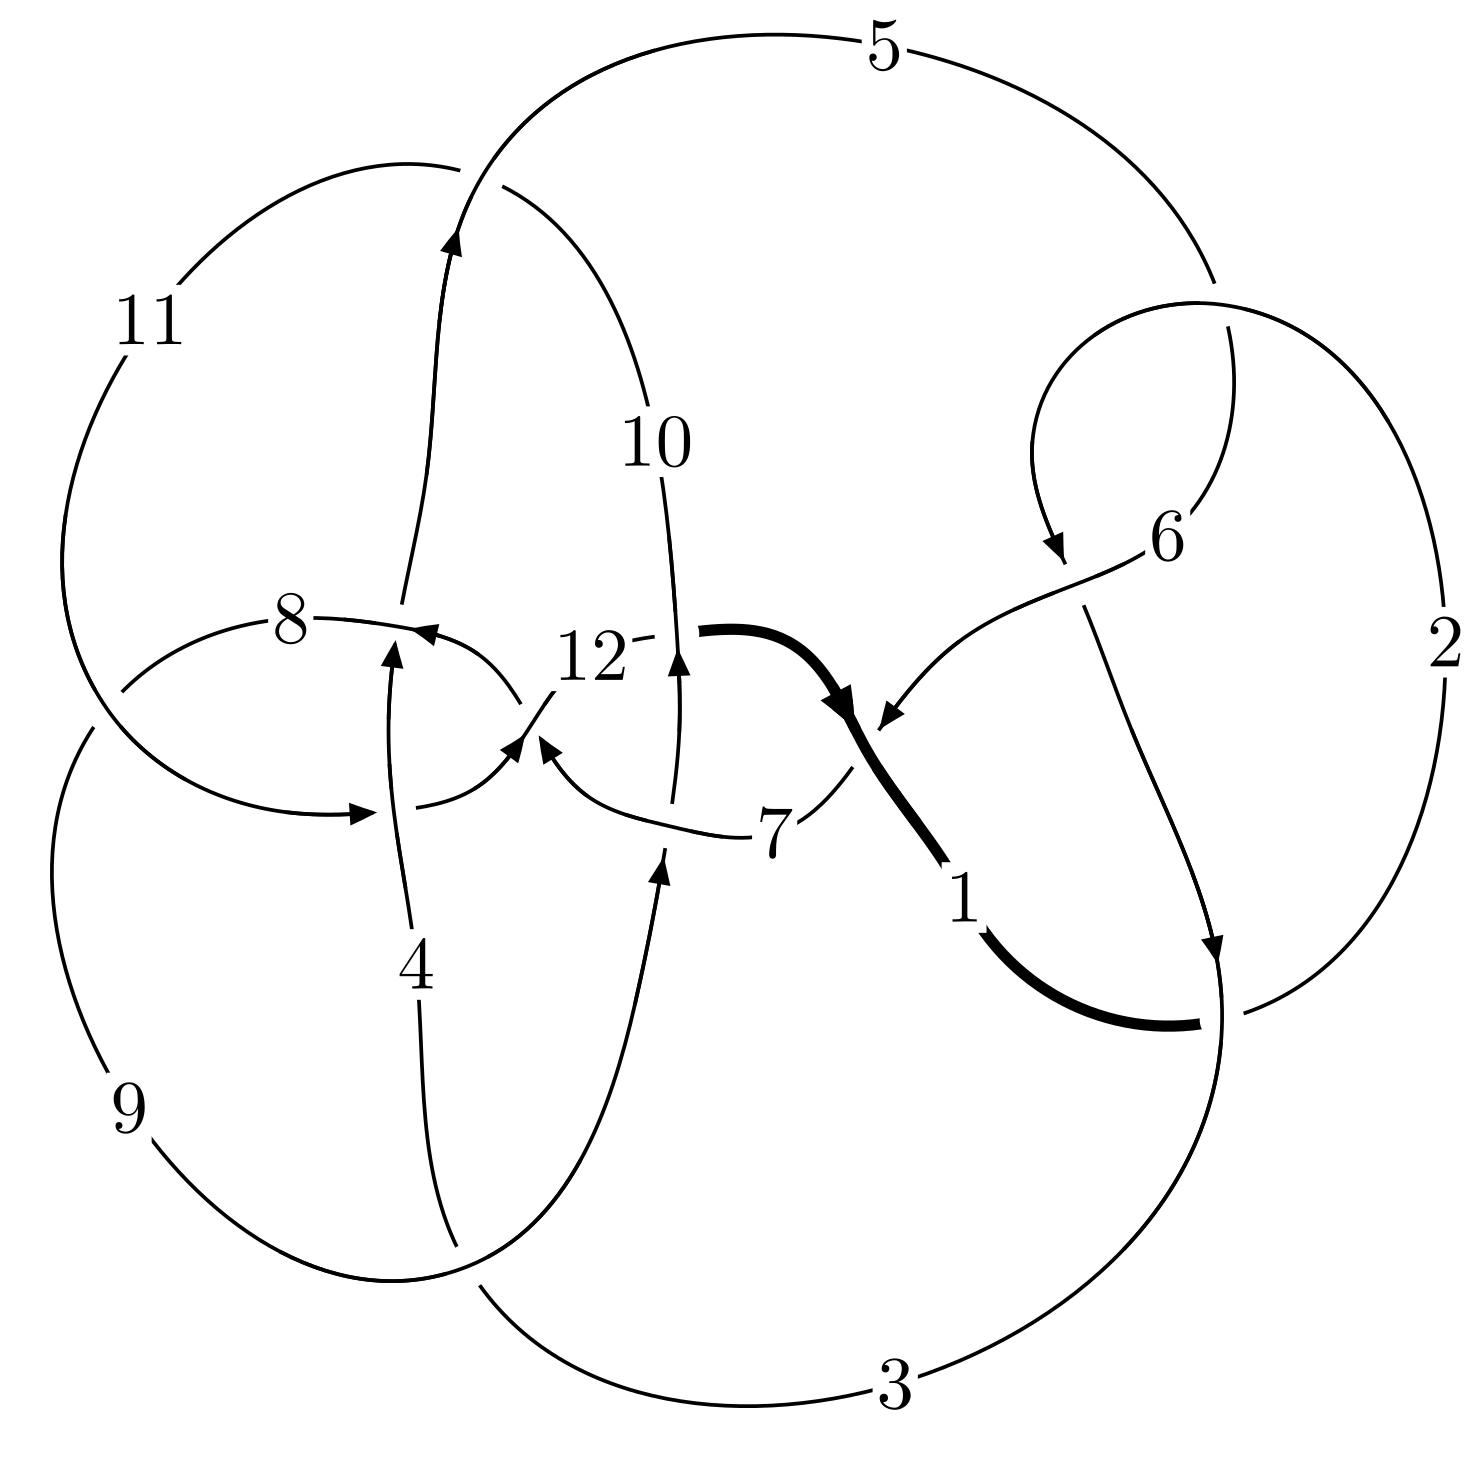
\includegraphics[width=112pt]{../../../GIT/diagram.site/Diagrams/png/1160_12a_0359.png}\\
\ \ \ A knot diagram\footnotemark}&
\allowdisplaybreaks
\textbf{Linearized knot diagam} \\
\cline{2-2}
 &
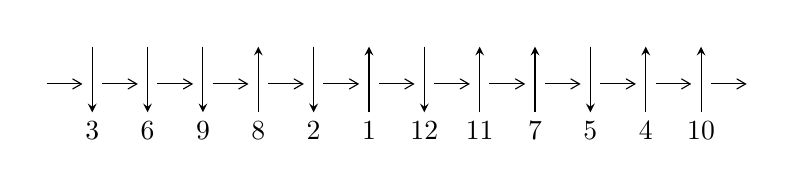
\begin{tikzpicture}[x=20pt, y=17pt]
	% nodes
	\node (C0) at (0, 0) {};
	\node (C1) at (1, 0) {};
	\node (C1U) at (1, +1) {};
	\node (C1D) at (1, -1) {3};

	\node (C2) at (2, 0) {};
	\node (C2U) at (2, +1) {};
	\node (C2D) at (2, -1) {6};

	\node (C3) at (3, 0) {};
	\node (C3U) at (3, +1) {};
	\node (C3D) at (3, -1) {9};

	\node (C4) at (4, 0) {};
	\node (C4U) at (4, +1) {};
	\node (C4D) at (4, -1) {8};

	\node (C5) at (5, 0) {};
	\node (C5U) at (5, +1) {};
	\node (C5D) at (5, -1) {2};

	\node (C6) at (6, 0) {};
	\node (C6U) at (6, +1) {};
	\node (C6D) at (6, -1) {1};

	\node (C7) at (7, 0) {};
	\node (C7U) at (7, +1) {};
	\node (C7D) at (7, -1) {12};

	\node (C8) at (8, 0) {};
	\node (C8U) at (8, +1) {};
	\node (C8D) at (8, -1) {11};

	\node (C9) at (9, 0) {};
	\node (C9U) at (9, +1) {};
	\node (C9D) at (9, -1) {7};

	\node (C10) at (10, 0) {};
	\node (C10U) at (10, +1) {};
	\node (C10D) at (10, -1) {5};

	\node (C11) at (11, 0) {};
	\node (C11U) at (11, +1) {};
	\node (C11D) at (11, -1) {4};

	\node (C12) at (12, 0) {};
	\node (C12U) at (12, +1) {};
	\node (C12D) at (12, -1) {10};
	\node (C13) at (13, 0) {};

	% arrows
	\draw[->,>={angle 60}]
	(C0) edge (C1) (C1) edge (C2) (C2) edge (C3) (C3) edge (C4) (C4) edge (C5) (C5) edge (C6) (C6) edge (C7) (C7) edge (C8) (C8) edge (C9) (C9) edge (C10) (C10) edge (C11) (C11) edge (C12) (C12) edge (C13) ;	\draw[->,>=stealth]
	(C1U) edge (C1D) (C2U) edge (C2D) (C3U) edge (C3D) (C4D) edge (C4U) (C5U) edge (C5D) (C6D) edge (C6U) (C7U) edge (C7D) (C8D) edge (C8U) (C9D) edge (C9U) (C10U) edge (C10D) (C11D) edge (C11U) (C12D) edge (C12U) ;
	\end{tikzpicture} \\
\hhline{~~} \\& 
\textbf{Solving Sequence} \\ \cline{2-2} 
 &
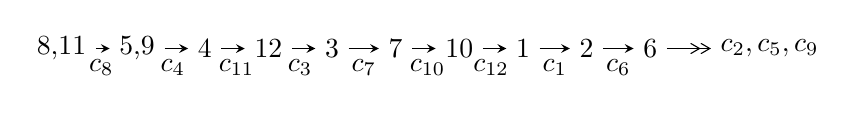
\begin{tikzpicture}[x=23pt, y=7pt]
	% node
	\node (A0) at (-1/8, 0) {8,11};
	\node (A1) at (17/16, 0) {5,9};
	\node (A2) at (17/8, 0) {4};
	\node (A3) at (25/8, 0) {12};
	\node (A4) at (33/8, 0) {3};
	\node (A5) at (41/8, 0) {7};
	\node (A6) at (49/8, 0) {10};
	\node (A7) at (57/8, 0) {1};
	\node (A8) at (65/8, 0) {2};
	\node (A9) at (73/8, 0) {6};
	\node (C1) at (1/2, -1) {$c_{8}$};
	\node (C2) at (13/8, -1) {$c_{4}$};
	\node (C3) at (21/8, -1) {$c_{11}$};
	\node (C4) at (29/8, -1) {$c_{3}$};
	\node (C5) at (37/8, -1) {$c_{7}$};
	\node (C6) at (45/8, -1) {$c_{10}$};
	\node (C7) at (53/8, -1) {$c_{12}$};
	\node (C8) at (61/8, -1) {$c_{1}$};
	\node (C9) at (69/8, -1) {$c_{6}$};
	\node (A10) at (11, 0) {$c_{2},c_{5},c_{9}$};

	% edge
	\draw[->,>=stealth]	
	(A0) edge (A1) (A1) edge (A2) (A2) edge (A3) (A3) edge (A4) (A4) edge (A5) (A5) edge (A6) (A6) edge (A7) (A7) edge (A8) (A8) edge (A9) ;
	\draw[->>,>={angle 60}]	
	(A9) edge (A10);
\end{tikzpicture} \\ 

\end{tabular} \\

\footnotetext{
The image of knot diagram is generated by the software ``\textbf{Draw programme}" developed by Andrew Bartholomew(\url{http://www.layer8.co.uk/maths/draw/index.htm\#Running-draw}), where we modified some parts for our purpose(\url{https://github.com/CATsTAILs/LinksPainter}).
}\phantom \\ \newline 
\centering \textbf{Ideals for irreducible components\footnotemark of $X_{\text{par}}$} 
 
\begin{align*}
I^u_{1}&=\langle 
-6.19368\times10^{103} u^{61}+2.38805\times10^{105} u^{60}+\cdots+6.33524\times10^{104} b-9.63557\times10^{103},\\
\phantom{I^u_{1}}&\phantom{= \langle  }-5.27642\times10^{103} u^{61}+2.16564\times10^{105} u^{60}+\cdots+2.11175\times10^{104} a+6.20998\times10^{104},\\
\phantom{I^u_{1}}&\phantom{= \langle  }u^{62}-42 u^{61}+\cdots+u+1\rangle \\
I^u_{2}&=\langle 
-583832 u^{30} a^3-50272 u^{30} a^2+\cdots-1355616 a-8946449,\;24 u^{30} a^3+144 u^{30} a^2+\cdots+838 a+793,\\
\phantom{I^u_{2}}&\phantom{= \langle  }u^{31}+15 u^{30}+\cdots+3 u+2\rangle \\
I^u_{3}&=\langle 
-4.46583\times10^{21} u^{31}-8.87689\times10^{22} u^{30}+\cdots+1.43348\times10^{22} b-3.51023\times10^{23},\\
\phantom{I^u_{3}}&\phantom{= \langle  }4.78754\times10^{22} u^{31}+8.67713\times10^{23} u^{30}+\cdots+7.16738\times10^{22} a+7.19257\times10^{23},\\
\phantom{I^u_{3}}&\phantom{= \langle  }u^{32}+19 u^{31}+\cdots+90 u+25\rangle \\
\\
I^v_{1}&=\langle 
a,\;b^2- b v+2 b- v+3,\;v^2-3 v+1\rangle \\
I^v_{2}&=\langle 
a,\;b^2- b+1,\;v-1\rangle \\
\end{align*}
\raggedright * 5 irreducible components of $\dim_{\mathbb{C}}=0$, with total 224 representations.\\
\footnotetext{All coefficients of polynomials are rational numbers. But the coefficients are sometimes approximated in decimal forms when there is not enough margin.}
\newpage
\renewcommand{\arraystretch}{1}
\centering \section*{I. $I^u_{1}= \langle -6.19\times10^{103} u^{61}+2.39\times10^{105} u^{60}+\cdots+6.34\times10^{104} b-9.64\times10^{103},\;-5.28\times10^{103} u^{61}+2.17\times10^{105} u^{60}+\cdots+2.11\times10^{104} a+6.21\times10^{104},\;u^{62}-42 u^{61}+\cdots+u+1 \rangle$}
\flushleft \textbf{(i) Arc colorings}\\
\begin{tabular}{m{7pt} m{180pt} m{7pt} m{180pt} }
\flushright $a_{8}=$&$\begin{pmatrix}1\\0\end{pmatrix}$ \\
\flushright $a_{11}=$&$\begin{pmatrix}0\\u\end{pmatrix}$ \\
\flushright $a_{5}=$&$\begin{pmatrix}0.249860 u^{61}-10.2552 u^{60}+\cdots-30.5916 u-2.94069\\0.0977655 u^{61}-3.76946 u^{60}+\cdots+3.24488 u+0.152095\end{pmatrix}$ \\
\flushright $a_{9}=$&$\begin{pmatrix}1\\- u^2\end{pmatrix}$ \\
\flushright $a_{4}=$&$\begin{pmatrix}0.152095 u^{61}-6.48575 u^{60}+\cdots-33.8365 u-3.09278\\0.0977655 u^{61}-3.76946 u^{60}+\cdots+3.24488 u+0.152095\end{pmatrix}$ \\
\flushright $a_{12}=$&$\begin{pmatrix}1.48851 u^{61}-61.9811 u^{60}+\cdots+9.74232 u+4.15415\\-0.536530 u^{61}+22.1350 u^{60}+\cdots-1.66564 u+1.48851\end{pmatrix}$ \\
\flushright $a_{3}=$&$\begin{pmatrix}-0.0868270 u^{61}+3.37589 u^{60}+\cdots-30.6459 u-2.84292\\0.0990411 u^{61}-4.06016 u^{60}+\cdots+2.83287 u-0.0209841\end{pmatrix}$ \\
\flushright $a_{7}=$&$\begin{pmatrix}0.368383 u^{61}-15.6825 u^{60}+\cdots-33.3998 u-3.23851\\0.609772 u^{61}-24.7449 u^{60}+\cdots+2.58185 u-0.168147\end{pmatrix}$ \\
\flushright $a_{10}=$&$\begin{pmatrix}0.814764 u^{61}-34.3056 u^{60}+\cdots+2.38599 u+6.59465\\-0.137220 u^{61}+5.54053 u^{60}+\cdots-3.69068 u+0.951984\end{pmatrix}$ \\
\flushright $a_{1}=$&$\begin{pmatrix}0.435369 u^{61}-17.8972 u^{60}+\cdots+35.4392 u+0.0678684\\-0.552957 u^{61}+22.6502 u^{60}+\cdots+0.563674 u+0.541616\end{pmatrix}$ \\
\flushright $a_{2}=$&$\begin{pmatrix}0.102413 u^{61}-4.15773 u^{60}+\cdots+39.1917 u+0.298157\\-0.224608 u^{61}+9.09838 u^{60}+\cdots-0.175732 u+0.131771\end{pmatrix}$ \\
\flushright $a_{6}=$&$\begin{pmatrix}0.0118368 u^{61}-0.600731 u^{60}+\cdots-38.9999 u-0.409916\\0.232933 u^{61}-9.64908 u^{60}+\cdots+0.103997 u-0.205997\end{pmatrix}$\\&\end{tabular}
\flushleft \textbf{(ii) Obstruction class $= -1$}\\~\\
\flushleft \textbf{(iii) Cusp Shapes $= -2.49621 u^{61}+103.028 u^{60}+\cdots-7.16311 u+4.09666$}\\~\\
\newpage\renewcommand{\arraystretch}{1}
\flushleft \textbf{(iv) u-Polynomials at the component}\newline \\
\begin{tabular}{m{50pt}|m{274pt}}
Crossings & \hspace{64pt}u-Polynomials at each crossing \\
\hline $$\begin{aligned}c_{1}\end{aligned}$$&$\begin{aligned}
&u^{62}+32 u^{61}+\cdots+25 u+1
\end{aligned}$\\
\hline $$\begin{aligned}c_{2},c_{5}\end{aligned}$$&$\begin{aligned}
&u^{62}+10 u^{61}+\cdots+9 u+1
\end{aligned}$\\
\hline $$\begin{aligned}c_{3},c_{10}\end{aligned}$$&$\begin{aligned}
&u^{62}+u^{61}+\cdots+157 u^2+9
\end{aligned}$\\
\hline $$\begin{aligned}c_{4},c_{11}\end{aligned}$$&$\begin{aligned}
&u^{62}+u^{61}+\cdots- u+1
\end{aligned}$\\
\hline $$\begin{aligned}c_{6}\end{aligned}$$&$\begin{aligned}
&u^{62}+30 u^{61}+\cdots+37547 u+2393
\end{aligned}$\\
\hline $$\begin{aligned}c_{7}\end{aligned}$$&$\begin{aligned}
&u^{62}+51 u^{61}+\cdots+30064771072 u+1073741824
\end{aligned}$\\
\hline $$\begin{aligned}c_{8}\end{aligned}$$&$\begin{aligned}
&u^{62}+42 u^{61}+\cdots- u+1
\end{aligned}$\\
\hline $$\begin{aligned}c_{9},c_{12}\end{aligned}$$&$\begin{aligned}
&u^{62}-3 u^{61}+\cdots-3 u+1
\end{aligned}$\\
\hline
\end{tabular}\\~\\
\newpage\renewcommand{\arraystretch}{1}
\flushleft \textbf{(v) Riley Polynomials at the component}\newline \\
\begin{tabular}{m{50pt}|m{274pt}}
Crossings & \hspace{64pt}Riley Polynomials at each crossing \\
\hline $$\begin{aligned}c_{1}\end{aligned}$$&$\begin{aligned}
&y^{62}+56 y^{60}+\cdots+127 y+1
\end{aligned}$\\
\hline $$\begin{aligned}c_{2},c_{5}\end{aligned}$$&$\begin{aligned}
&y^{62}-32 y^{61}+\cdots-25 y+1
\end{aligned}$\\
\hline $$\begin{aligned}c_{3},c_{10}\end{aligned}$$&$\begin{aligned}
&y^{62}+21 y^{61}+\cdots+2826 y+81
\end{aligned}$\\
\hline $$\begin{aligned}c_{4},c_{11}\end{aligned}$$&$\begin{aligned}
&y^{62}+9 y^{61}+\cdots+17 y+1
\end{aligned}$\\
\hline $$\begin{aligned}c_{6}\end{aligned}$$&$\begin{aligned}
&y^{62}+26 y^{61}+\cdots-77618039 y+5726449
\end{aligned}$\\
\hline $$\begin{aligned}c_{7}\end{aligned}$$&$\begin{aligned}
&y^{62}+19 y^{61}+\cdots-1.15\times10^{18} y+1.15\times10^{18}
\end{aligned}$\\
\hline $$\begin{aligned}c_{8}\end{aligned}$$&$\begin{aligned}
&y^{62}-8 y^{61}+\cdots-51 y+1
\end{aligned}$\\
\hline $$\begin{aligned}c_{9},c_{12}\end{aligned}$$&$\begin{aligned}
&y^{62}+21 y^{61}+\cdots+y+1
\end{aligned}$\\
\hline
\end{tabular}\\~\\
\newpage\flushleft \textbf{(vi) Complex Volumes and Cusp Shapes}
$$\begin{array}{c|c|c}  
\text{Solutions to }I^u_{1}& \I (\text{vol} + \sqrt{-1}CS) & \text{Cusp shape}\\
 \hline 
\begin{aligned}
u &= \phantom{-}0.920164 + 0.258178 I \\
a &= -0.171522 - 0.193932 I \\
b &= -0.669614 + 0.624449 I\end{aligned}
 & -2.59019 - 4.63724 I & \phantom{-0.000000 } 0 \\ \hline\begin{aligned}
u &= \phantom{-}0.920164 - 0.258178 I \\
a &= -0.171522 + 0.193932 I \\
b &= -0.669614 - 0.624449 I\end{aligned}
 & -2.59019 + 4.63724 I & \phantom{-0.000000 } 0 \\ \hline\begin{aligned}
u &= \phantom{-}0.499373 + 0.963398 I \\
a &= \phantom{-}0.438750 - 0.923022 I \\
b &= -0.501971 - 0.889599 I\end{aligned}
 & -3.88281 - 0.46065 I & \phantom{-0.000000 } 0 \\ \hline\begin{aligned}
u &= \phantom{-}0.499373 - 0.963398 I \\
a &= \phantom{-}0.438750 + 0.923022 I \\
b &= -0.501971 + 0.889599 I\end{aligned}
 & -3.88281 + 0.46065 I & \phantom{-0.000000 } 0 \\ \hline\begin{aligned}
u &= \phantom{-}0.979389 + 0.514465 I \\
a &= -0.220792 + 0.721446 I \\
b &= \phantom{-}1.19645 + 1.09383 I\end{aligned}
 & \phantom{-}1.85971 + 4.94822 I & \phantom{-0.000000 } 0 \\ \hline\begin{aligned}
u &= \phantom{-}0.979389 - 0.514465 I \\
a &= -0.220792 - 0.721446 I \\
b &= \phantom{-}1.19645 - 1.09383 I\end{aligned}
 & \phantom{-}1.85971 - 4.94822 I & \phantom{-0.000000 } 0 \\ \hline\begin{aligned}
u &= \phantom{-}0.438857 + 1.057020 I \\
a &= -0.410593 + 1.007440 I \\
b &= \phantom{-}0.493823 + 0.915752 I\end{aligned}
 & -6.71452 - 5.10423 I & \phantom{-0.000000 } 0 \\ \hline\begin{aligned}
u &= \phantom{-}0.438857 - 1.057020 I \\
a &= -0.410593 - 1.007440 I \\
b &= \phantom{-}0.493823 - 0.915752 I\end{aligned}
 & -6.71452 + 5.10423 I & \phantom{-0.000000 } 0 \\ \hline\begin{aligned}
u &= \phantom{-}0.888552 + 0.744591 I \\
a &= \phantom{-}0.185048 - 0.989964 I \\
b &= -1.15174 - 1.03840 I\end{aligned}
 & -2.92298 + 9.42642 I & \phantom{-0.000000 } 0 \\ \hline\begin{aligned}
u &= \phantom{-}0.888552 - 0.744591 I \\
a &= \phantom{-}0.185048 + 0.989964 I \\
b &= -1.15174 + 1.03840 I\end{aligned}
 & -2.92298 - 9.42642 I & \phantom{-0.000000 } 0\\
 \hline 
 \end{array}$$\newpage$$\begin{array}{c|c|c}  
\text{Solutions to }I^u_{1}& \I (\text{vol} + \sqrt{-1}CS) & \text{Cusp shape}\\
 \hline 
\begin{aligned}
u &= \phantom{-}0.629220 + 1.055740 I \\
a &= -0.319267 + 0.898480 I \\
b &= \phantom{-}0.532879 + 0.901613 I\end{aligned}
 & -7.79004 + 3.14172 I & \phantom{-0.000000 } 0 \\ \hline\begin{aligned}
u &= \phantom{-}0.629220 - 1.055740 I \\
a &= -0.319267 - 0.898480 I \\
b &= \phantom{-}0.532879 - 0.901613 I\end{aligned}
 & -7.79004 - 3.14172 I & \phantom{-0.000000 } 0 \\ \hline\begin{aligned}
u &= \phantom{-}1.234050 + 0.374671 I \\
a &= \phantom{-}0.014869 - 0.420306 I \\
b &= -0.774223 - 0.952918 I\end{aligned}
 & -0.34790 - 1.71219 I & \phantom{-0.000000 } 0 \\ \hline\begin{aligned}
u &= \phantom{-}1.234050 - 0.374671 I \\
a &= \phantom{-}0.014869 + 0.420306 I \\
b &= -0.774223 + 0.952918 I\end{aligned}
 & -0.34790 + 1.71219 I & \phantom{-0.000000 } 0 \\ \hline\begin{aligned}
u &= \phantom{-}0.541110 + 0.364429 I \\
a &= \phantom{-}0.919250 - 0.771221 I \\
b &= -1.127670 - 0.716169 I\end{aligned}
 & -2.36554 - 0.52359 I & \phantom{-0.000000 } 0 \\ \hline\begin{aligned}
u &= \phantom{-}0.541110 - 0.364429 I \\
a &= \phantom{-}0.919250 + 0.771221 I \\
b &= -1.127670 + 0.716169 I\end{aligned}
 & -2.36554 + 0.52359 I & \phantom{-0.000000 } 0 \\ \hline\begin{aligned}
u &= -0.226942 + 0.567500 I \\
a &= -1.15526 + 1.37476 I \\
b &= \phantom{-}0.047302 + 0.810504 I\end{aligned}
 & -3.30081 + 1.51078 I & \phantom{-0.000000 } 0 \\ \hline\begin{aligned}
u &= -0.226942 - 0.567500 I \\
a &= -1.15526 - 1.37476 I \\
b &= \phantom{-}0.047302 - 0.810504 I\end{aligned}
 & -3.30081 - 1.51078 I & \phantom{-0.000000 } 0 \\ \hline\begin{aligned}
u &= \phantom{-}1.34172 + 0.51463 I \\
a &= -0.055225 + 0.493349 I \\
b &= \phantom{-}0.560633 + 1.009600 I\end{aligned}
 & \phantom{-}1.18701 + 3.96993 I & \phantom{-0.000000 } 0 \\ \hline\begin{aligned}
u &= \phantom{-}1.34172 - 0.51463 I \\
a &= -0.055225 - 0.493349 I \\
b &= \phantom{-}0.560633 - 1.009600 I\end{aligned}
 & \phantom{-}1.18701 - 3.96993 I & \phantom{-0.000000 } 0\\
 \hline 
 \end{array}$$\newpage$$\begin{array}{c|c|c}  
\text{Solutions to }I^u_{1}& \I (\text{vol} + \sqrt{-1}CS) & \text{Cusp shape}\\
 \hline 
\begin{aligned}
u &= -0.317222 + 0.464851 I \\
a &= -1.54500 + 1.62152 I \\
b &= -0.115660 + 0.894922 I\end{aligned}
 & -2.78728 - 5.95527 I & -4.95646 + 7.62237 I \\ \hline\begin{aligned}
u &= -0.317222 - 0.464851 I \\
a &= -1.54500 - 1.62152 I \\
b &= -0.115660 - 0.894922 I\end{aligned}
 & -2.78728 + 5.95527 I & -4.95646 - 7.62237 I \\ \hline\begin{aligned}
u &= \phantom{-}0.249047 + 0.492818 I \\
a &= \phantom{-}1.049160 - 0.849645 I \\
b &= -0.446366 - 0.699671 I\end{aligned}
 & -1.63065 - 0.67826 I & -5.63896 + 2.73445 I \\ \hline\begin{aligned}
u &= \phantom{-}0.249047 - 0.492818 I \\
a &= \phantom{-}1.049160 + 0.849645 I \\
b &= -0.446366 + 0.699671 I\end{aligned}
 & -1.63065 + 0.67826 I & -5.63896 - 2.73445 I \\ \hline\begin{aligned}
u &= -0.203334 + 0.491918 I \\
a &= \phantom{-}1.53789 - 0.98833 I \\
b &= \phantom{-}0.155182 - 0.732250 I\end{aligned}
 & -0.19950 - 1.86693 I & -1.22584 + 4.41138 I \\ \hline\begin{aligned}
u &= -0.203334 - 0.491918 I \\
a &= \phantom{-}1.53789 + 0.98833 I \\
b &= \phantom{-}0.155182 + 0.732250 I\end{aligned}
 & -0.19950 + 1.86693 I & -1.22584 - 4.41138 I \\ \hline\begin{aligned}
u &= \phantom{-}1.19510 + 0.85598 I \\
a &= \phantom{-}0.111753 + 0.918781 I \\
b &= \phantom{-}1.16040 + 1.02724 I\end{aligned}
 & \phantom{-}5.91226 + 7.99963 I & \phantom{-0.000000 } 0 \\ \hline\begin{aligned}
u &= \phantom{-}1.19510 - 0.85598 I \\
a &= \phantom{-}0.111753 - 0.918781 I \\
b &= \phantom{-}1.16040 - 1.02724 I\end{aligned}
 & \phantom{-}5.91226 - 7.99963 I & \phantom{-0.000000 } 0 \\ \hline\begin{aligned}
u &= \phantom{-}1.20252 + 0.93906 I \\
a &= -0.152053 - 0.972240 I \\
b &= -1.17474 - 1.03088 I\end{aligned}
 & \phantom{-}6.0483 + 13.4168 I & \phantom{-0.000000 } 0 \\ \hline\begin{aligned}
u &= \phantom{-}1.20252 - 0.93906 I \\
a &= -0.152053 + 0.972240 I \\
b &= -1.17474 + 1.03088 I\end{aligned}
 & \phantom{-}6.0483 - 13.4168 I & \phantom{-0.000000 } 0\\
 \hline 
 \end{array}$$\newpage$$\begin{array}{c|c|c}  
\text{Solutions to }I^u_{1}& \I (\text{vol} + \sqrt{-1}CS) & \text{Cusp shape}\\
 \hline 
\begin{aligned}
u &= \phantom{-}1.10244 + 1.06100 I \\
a &= \phantom{-}0.146064 + 1.095100 I \\
b &= \phantom{-}1.18184 + 1.05744 I\end{aligned}
 & -1.67279 + 12.65800 I & \phantom{-0.000000 } 0 \\ \hline\begin{aligned}
u &= \phantom{-}1.10244 - 1.06100 I \\
a &= \phantom{-}0.146064 - 1.095100 I \\
b &= \phantom{-}1.18184 - 1.05744 I\end{aligned}
 & -1.67279 - 12.65800 I & \phantom{-0.000000 } 0 \\ \hline\begin{aligned}
u &= -1.48802 + 0.48856 I \\
a &= \phantom{-}0.139890 - 0.500048 I \\
b &= \phantom{-}0.047752 - 0.317158 I\end{aligned}
 & \phantom{-}2.20261 - 2.33406 I & \phantom{-0.000000 } 0 \\ \hline\begin{aligned}
u &= -1.48802 - 0.48856 I \\
a &= \phantom{-}0.139890 + 0.500048 I \\
b &= \phantom{-}0.047752 + 0.317158 I\end{aligned}
 & \phantom{-}2.20261 + 2.33406 I & \phantom{-0.000000 } 0 \\ \hline\begin{aligned}
u &= \phantom{-}1.21760 + 1.00691 I \\
a &= \phantom{-}0.063374 - 0.672036 I \\
b &= -0.561277 - 0.869964 I\end{aligned}
 & -5.76493 + 4.37566 I & \phantom{-0.000000 } 0 \\ \hline\begin{aligned}
u &= \phantom{-}1.21760 - 1.00691 I \\
a &= \phantom{-}0.063374 + 0.672036 I \\
b &= -0.561277 + 0.869964 I\end{aligned}
 & -5.76493 - 4.37566 I & \phantom{-0.000000 } 0 \\ \hline\begin{aligned}
u &= \phantom{-}1.16698 + 1.07593 I \\
a &= -0.191200 - 1.072920 I \\
b &= -1.19188 - 1.05052 I\end{aligned}
 & \phantom{-}3.2276 + 16.0824 I & \phantom{-0.000000 } 0 \\ \hline\begin{aligned}
u &= \phantom{-}1.16698 - 1.07593 I \\
a &= -0.191200 + 1.072920 I \\
b &= -1.19188 + 1.05052 I\end{aligned}
 & \phantom{-}3.2276 - 16.0824 I & \phantom{-0.000000 } 0 \\ \hline\begin{aligned}
u &= \phantom{-}1.16841 + 1.11208 I \\
a &= \phantom{-}0.208737 + 1.092990 I \\
b &= \phantom{-}1.19732 + 1.05500 I\end{aligned}
 & \phantom{-}0.5718 + 21.3392 I & \phantom{-0.000000 } 0 \\ \hline\begin{aligned}
u &= \phantom{-}1.16841 - 1.11208 I \\
a &= \phantom{-}0.208737 - 1.092990 I \\
b &= \phantom{-}1.19732 - 1.05500 I\end{aligned}
 & \phantom{-}0.5718 - 21.3392 I & \phantom{-0.000000 } 0\\
 \hline 
 \end{array}$$\newpage$$\begin{array}{c|c|c}  
\text{Solutions to }I^u_{1}& \I (\text{vol} + \sqrt{-1}CS) & \text{Cusp shape}\\
 \hline 
\begin{aligned}
u &= -0.326655 + 0.081761 I \\
a &= -1.01998 - 4.35874 I \\
b &= -0.455772 - 1.038460 I\end{aligned}
 & -2.34446 - 1.67897 I & -3.97540 + 0.64256 I \\ \hline\begin{aligned}
u &= -0.326655 - 0.081761 I \\
a &= -1.01998 + 4.35874 I \\
b &= -0.455772 + 1.038460 I\end{aligned}
 & -2.34446 + 1.67897 I & -3.97540 - 0.64256 I \\ \hline\begin{aligned}
u &= -0.238513 + 0.230540 I \\
a &= \phantom{-}0.43580 - 4.41695 I \\
b &= -0.545904 - 1.033350 I\end{aligned}
 & -2.44610 + 5.55793 I & -3.92344 - 7.42769 I \\ \hline\begin{aligned}
u &= -0.238513 - 0.230540 I \\
a &= \phantom{-}0.43580 + 4.41695 I \\
b &= -0.545904 + 1.033350 I\end{aligned}
 & -2.44610 - 5.55793 I & -3.92344 + 7.42769 I \\ \hline\begin{aligned}
u &= \phantom{-}1.30406 + 1.14133 I \\
a &= \phantom{-}0.495631 + 0.091161 I \\
b &= \phantom{-}0.678233 - 0.294448 I\end{aligned}
 & -1.69191 - 4.30137 I & \phantom{-0.000000 } 0 \\ \hline\begin{aligned}
u &= \phantom{-}1.30406 - 1.14133 I \\
a &= \phantom{-}0.495631 - 0.091161 I \\
b &= \phantom{-}0.678233 + 0.294448 I\end{aligned}
 & -1.69191 + 4.30137 I & \phantom{-0.000000 } 0 \\ \hline\begin{aligned}
u &= \phantom{-}1.43507 + 1.00279 I \\
a &= \phantom{-}0.006386 + 0.624885 I \\
b &= \phantom{-}0.533141 + 0.847055 I\end{aligned}
 & -0.63962 + 7.41146 I & \phantom{-0.000000 } 0 \\ \hline\begin{aligned}
u &= \phantom{-}1.43507 - 1.00279 I \\
a &= \phantom{-}0.006386 - 0.624885 I \\
b &= \phantom{-}0.533141 - 0.847055 I\end{aligned}
 & -0.63962 - 7.41146 I & \phantom{-0.000000 } 0 \\ \hline\begin{aligned}
u &= \phantom{-}1.44646 + 1.10837 I \\
a &= -0.032947 - 0.651358 I \\
b &= -0.548879 - 0.829457 I\end{aligned}
 & -3.10035 + 12.75660 I & \phantom{-0.000000 } 0 \\ \hline\begin{aligned}
u &= \phantom{-}1.44646 - 1.10837 I \\
a &= -0.032947 + 0.651358 I \\
b &= -0.548879 + 0.829457 I\end{aligned}
 & -3.10035 - 12.75660 I & \phantom{-0.000000 } 0\\
 \hline 
 \end{array}$$\newpage$$\begin{array}{c|c|c}  
\text{Solutions to }I^u_{1}& \I (\text{vol} + \sqrt{-1}CS) & \text{Cusp shape}\\
 \hline 
\begin{aligned}
u &= \phantom{-}0.059087 + 0.137841 I \\
a &= -6.27225 + 2.11029 I \\
b &= \phantom{-}0.575488 + 0.870652 I\end{aligned}
 & -0.00632 + 2.04316 I & \phantom{-}0.51473 - 3.73697 I \\ \hline\begin{aligned}
u &= \phantom{-}0.059087 - 0.137841 I \\
a &= -6.27225 - 2.11029 I \\
b &= \phantom{-}0.575488 - 0.870652 I\end{aligned}
 & -0.00632 - 2.04316 I & \phantom{-}0.51473 + 3.73697 I \\ \hline\begin{aligned}
u &= -0.1162010 + 0.0391791 I \\
a &= \phantom{-}6.30651 - 6.74361 I \\
b &= \phantom{-}0.451685 - 0.907545 I\end{aligned}
 & \phantom{-}0.00633 - 2.03596 I & \phantom{-}0.03927 + 3.79777 I \\ \hline\begin{aligned}
u &= -0.1162010 - 0.0391791 I \\
a &= \phantom{-}6.30651 + 6.74361 I \\
b &= \phantom{-}0.451685 + 0.907545 I\end{aligned}
 & \phantom{-}0.00633 + 2.03596 I & \phantom{-}0.03927 - 3.79777 I \\ \hline\begin{aligned}
u &= \phantom{-}1.42808 + 1.37693 I \\
a &= -0.496587 - 0.104373 I \\
b &= -0.667948 + 0.203001 I\end{aligned}
 & \phantom{-}2.88874 - 7.13321 I & \phantom{-0.000000 } 0 \\ \hline\begin{aligned}
u &= \phantom{-}1.42808 - 1.37693 I \\
a &= -0.496587 + 0.104373 I \\
b &= -0.667948 - 0.203001 I\end{aligned}
 & \phantom{-}2.88874 + 7.13321 I & \phantom{-0.000000 } 0 \\ \hline\begin{aligned}
u &= \phantom{-}1.53493 + 1.32200 I \\
a &= \phantom{-}0.507691 + 0.106764 I \\
b &= \phantom{-}0.710619 - 0.195157 I\end{aligned}
 & \phantom{-}0.49623 - 12.18690 I & \phantom{-0.000000 } 0 \\ \hline\begin{aligned}
u &= \phantom{-}1.53493 - 1.32200 I \\
a &= \phantom{-}0.507691 - 0.106764 I \\
b &= \phantom{-}0.710619 + 0.195157 I\end{aligned}
 & \phantom{-}0.49623 + 12.18690 I & \phantom{-0.000000 } 0 \\ \hline\begin{aligned}
u &= \phantom{-}1.11399 + 1.72823 I \\
a &= -0.462115 - 0.079137 I \\
b &= -0.525267 + 0.184090 I\end{aligned}
 & \phantom{-}4.48939 - 4.83470 I & \phantom{-0.000000 } 0 \\ \hline\begin{aligned}
u &= \phantom{-}1.11399 - 1.72823 I \\
a &= -0.462115 + 0.079137 I \\
b &= -0.525267 - 0.184090 I\end{aligned}
 & \phantom{-}4.48939 + 4.83470 I & \phantom{-0.000000 } 0\\
 \hline 
 \end{array}$$\newpage$$\begin{array}{c|c|c}  
\text{Solutions to }I^u_{1}& \I (\text{vol} + \sqrt{-1}CS) & \text{Cusp shape}\\
 \hline 
\begin{aligned}
u &= \phantom{-}0.82068 + 1.97978 I \\
a &= \phantom{-}0.437989 + 0.036032 I \\
b &= \phantom{-}0.436166 - 0.185034 I\end{aligned}
 & \phantom{-}3.56951 + 0.16849 I & \phantom{-0.000000 } 0 \\ \hline\begin{aligned}
u &= \phantom{-}0.82068 - 1.97978 I \\
a &= \phantom{-}0.437989 - 0.036032 I \\
b &= \phantom{-}0.436166 + 0.185034 I\end{aligned}
 & \phantom{-}3.56951 - 0.16849 I & \phantom{-0.000000 } 0\\
 \hline 
 \end{array}$$\newpage\newpage\renewcommand{\arraystretch}{1}
\centering \section*{II. $I^u_{2}= \langle -5.84\times10^{5} a^{3} u^{30}-5.03\times10^{4} a^{2} u^{30}+\cdots-1.36\times10^{6} a-8.95\times10^{6},\;24 u^{30} a^3+144 u^{30} a^2+\cdots+838 a+793,\;u^{31}+15 u^{30}+\cdots+3 u+2 \rangle$}
\flushleft \textbf{(i) Arc colorings}\\
\begin{tabular}{m{7pt} m{180pt} m{7pt} m{180pt} }
\flushright $a_{8}=$&$\begin{pmatrix}1\\0\end{pmatrix}$ \\
\flushright $a_{11}=$&$\begin{pmatrix}0\\u\end{pmatrix}$ \\
\flushright $a_{5}=$&$\begin{pmatrix}a\\0.495299 a^{3} u^{30}+0.0426487 a^{2} u^{30}+\cdots+1.15005 a+7.58980\end{pmatrix}$ \\
\flushright $a_{9}=$&$\begin{pmatrix}1\\- u^2\end{pmatrix}$ \\
\flushright $a_{4}=$&$\begin{pmatrix}-0.495299 a^{3} u^{30}-0.0426487 a^{2} u^{30}+\cdots-0.150049 a-7.58980\\0.495299 a^{3} u^{30}+0.0426487 a^{2} u^{30}+\cdots+1.15005 a+7.58980\end{pmatrix}$ \\
\flushright $a_{12}=$&$\begin{pmatrix}-0.121390 a^{3} u^{30}-0.530815 a^{2} u^{30}+\cdots+0.594693 a-2.19483\\0.0787413 a^{3} u^{30}-0.0221048 a^{2} u^{30}+\cdots+1.82404 a-0.212522\end{pmatrix}$ \\
\flushright $a_{3}=$&$\begin{pmatrix}-0.898170 a^{3} u^{30}+0.878610 a^{2} u^{30}+\cdots+0.903562 a-1.36728\\1.92968 a^{3} u^{30}-1.83328 a^{2} u^{30}+\cdots+3.91158 a+5.36658\end{pmatrix}$ \\
\flushright $a_{7}=$&$\begin{pmatrix}0.0407111 a^{3} u^{30}-0.535162 a^{2} u^{30}+\cdots-3.84252 a-2.55769\\0.0787413 a^{3} u^{30}-0.0221048 a^{2} u^{30}+\cdots+1.82404 a+0.787478\end{pmatrix}$ \\
\flushright $a_{10}=$&$\begin{pmatrix}a^2 u\\0.0426487 a^{3} u^{30}+0.552920 a^{2} u^{30}+\cdots-2.41874 a+2.40735\end{pmatrix}$ \\
\flushright $a_{1}=$&$\begin{pmatrix}0.00461847 a^{3} u^{30}-0.960137 a^{2} u^{30}+\cdots-2.08530 a-1.93781\\-2.09453 a^{3} u^{30}+1.81444 a^{2} u^{30}+\cdots-4.99193 a+4.06092\end{pmatrix}$ \\
\flushright $a_{2}=$&$\begin{pmatrix}0.953931 a^{3} u^{30}-0.775684 a^{2} u^{30}+\cdots-1.46886 a-2.39151\\-3.38652 a^{3} u^{30}+1.47922 a^{2} u^{30}+\cdots-3.39276 a+4.99159\end{pmatrix}$ \\
\flushright $a_{6}=$&$\begin{pmatrix}-1.13256 a^{3} u^{30}+0.301378 a^{2} u^{30}+\cdots-0.658493 a+0.715757\\0.609317 a^{3} u^{30}-0.0145222 a^{2} u^{30}+\cdots-2.67703 a-5.87958\end{pmatrix}$\\&\end{tabular}
\flushleft \textbf{(ii) Obstruction class $= -1$}\\~\\
\flushleft \textbf{(iii) Cusp Shapes $= -\frac{185632}{589373} u^{30} a^3+\frac{52112}{589373} u^{30} a^2+\cdots-\frac{4300168}{589373} a+\frac{19950327}{589373}$}\\~\\
\newpage\renewcommand{\arraystretch}{1}
\flushleft \textbf{(iv) u-Polynomials at the component}\newline \\
\begin{tabular}{m{50pt}|m{274pt}}
Crossings & \hspace{64pt}u-Polynomials at each crossing \\
\hline $$\begin{aligned}c_{1}\end{aligned}$$&$\begin{aligned}
&(u^{31}+16 u^{30}+\cdots+2 u+1)^{4}
\end{aligned}$\\
\hline $$\begin{aligned}c_{2},c_{5}\end{aligned}$$&$\begin{aligned}
&(u^{31}-2 u^{30}+\cdots-2 u+1)^{4}
\end{aligned}$\\
\hline $$\begin{aligned}c_{3},c_{10}\end{aligned}$$&$\begin{aligned}
&u^{124}+2 u^{123}+\cdots+445543889 u+54599377
\end{aligned}$\\
\hline $$\begin{aligned}c_{4},c_{11}\end{aligned}$$&$\begin{aligned}
&u^{124}+2 u^{123}+\cdots- u+1
\end{aligned}$\\
\hline $$\begin{aligned}c_{6}\end{aligned}$$&$\begin{aligned}
&(u^{31}-9 u^{30}+\cdots+73 u-8)^{4}
\end{aligned}$\\
\hline $$\begin{aligned}c_{7}\end{aligned}$$&$\begin{aligned}
&(u^2- u+1)^{62}
\end{aligned}$\\
\hline $$\begin{aligned}c_{8}\end{aligned}$$&$\begin{aligned}
&(u^{31}-15 u^{30}+\cdots+3 u-2)^{4}
\end{aligned}$\\
\hline $$\begin{aligned}c_{9},c_{12}\end{aligned}$$&$\begin{aligned}
&u^{124}-3 u^{123}+\cdots+54 u+1
\end{aligned}$\\
\hline
\end{tabular}\\~\\
\newpage\renewcommand{\arraystretch}{1}
\flushleft \textbf{(v) Riley Polynomials at the component}\newline \\
\begin{tabular}{m{50pt}|m{274pt}}
Crossings & \hspace{64pt}Riley Polynomials at each crossing \\
\hline $$\begin{aligned}c_{1}\end{aligned}$$&$\begin{aligned}
&(y^{31}+28 y^{29}+\cdots-14 y-1)^{4}
\end{aligned}$\\
\hline $$\begin{aligned}c_{2},c_{5}\end{aligned}$$&$\begin{aligned}
&(y^{31}-16 y^{30}+\cdots+2 y-1)^{4}
\end{aligned}$\\
\hline $$\begin{aligned}c_{3},c_{10}\end{aligned}$$&$\begin{aligned}
&y^{124}+42 y^{123}+\cdots-6608919476226557 y+2981091968788129
\end{aligned}$\\
\hline $$\begin{aligned}c_{4},c_{11}\end{aligned}$$&$\begin{aligned}
&y^{124}-42 y^{123}+\cdots+283 y+1
\end{aligned}$\\
\hline $$\begin{aligned}c_{6}\end{aligned}$$&$\begin{aligned}
&(y^{31}+13 y^{30}+\cdots+833 y-64)^{4}
\end{aligned}$\\
\hline $$\begin{aligned}c_{7}\end{aligned}$$&$\begin{aligned}
&(y^2+y+1)^{62}
\end{aligned}$\\
\hline $$\begin{aligned}c_{8}\end{aligned}$$&$\begin{aligned}
&(y^{31}-3 y^{30}+\cdots+69 y-4)^{4}
\end{aligned}$\\
\hline $$\begin{aligned}c_{9},c_{12}\end{aligned}$$&$\begin{aligned}
&y^{124}-31 y^{123}+\cdots-498 y+1
\end{aligned}$\\
\hline
\end{tabular}\\~\\
\newpage\flushleft \textbf{(vi) Complex Volumes and Cusp Shapes}
$$\begin{array}{c|c|c}  
\text{Solutions to }I^u_{2}& \I (\text{vol} + \sqrt{-1}CS) & \text{Cusp shape}\\
 \hline 
\begin{aligned}
u &= -0.409801 + 0.900274 I \\
a &= -0.506789 + 0.851719 I \\
b &= -1.53214 + 0.83196 I\end{aligned}
 & -0.60079 - 6.55319 I & -2.41907 + 9.71050 I \\ \hline\begin{aligned}
u &= -0.409801 + 0.900274 I \\
a &= \phantom{-}0.534702 - 0.939505 I \\
b &= \phantom{-}0.603624 - 0.987957 I\end{aligned}
 & -0.60079 - 2.49343 I & -2.41907 + 2.78230 I \\ \hline\begin{aligned}
u &= -0.409801 + 0.900274 I \\
a &= \phantom{-}1.177230 + 0.223519 I \\
b &= \phantom{-}0.0153756 + 0.0819040 I\end{aligned}
 & -0.60079 - 2.49343 I & -2.41907 + 2.78230 I \\ \hline\begin{aligned}
u &= -0.409801 + 0.900274 I \\
a &= -0.96924 - 1.97631 I \\
b &= \phantom{-}0.437980 - 0.915004 I\end{aligned}
 & -0.60079 - 6.55319 I & -2.41907 + 9.71050 I \\ \hline\begin{aligned}
u &= -0.409801 - 0.900274 I \\
a &= -0.506789 - 0.851719 I \\
b &= -1.53214 - 0.83196 I\end{aligned}
 & -0.60079 + 6.55319 I & -2.41907 - 9.71050 I \\ \hline\begin{aligned}
u &= -0.409801 - 0.900274 I \\
a &= \phantom{-}0.534702 + 0.939505 I \\
b &= \phantom{-}0.603624 + 0.987957 I\end{aligned}
 & -0.60079 + 2.49343 I & -2.41907 - 2.78230 I \\ \hline\begin{aligned}
u &= -0.409801 - 0.900274 I \\
a &= \phantom{-}1.177230 - 0.223519 I \\
b &= \phantom{-}0.0153756 - 0.0819040 I\end{aligned}
 & -0.60079 + 2.49343 I & -2.41907 - 2.78230 I \\ \hline\begin{aligned}
u &= -0.409801 - 0.900274 I \\
a &= -0.96924 + 1.97631 I \\
b &= \phantom{-}0.437980 + 0.915004 I\end{aligned}
 & -0.60079 + 6.55319 I & -2.41907 - 9.71050 I \\ \hline\begin{aligned}
u &= -1.020150 + 0.219444 I \\
a &= \phantom{-}0.137660 + 1.011220 I \\
b &= -0.599567 - 0.078037 I\end{aligned}
 & \phantom{-}3.66483 + 1.12535 I & \phantom{-}9.65108 - 2.67079 I \\ \hline\begin{aligned}
u &= -1.020150 + 0.219444 I \\
a &= \phantom{-}0.542247 - 0.929539 I \\
b &= \phantom{-}1.23471 - 1.06885 I\end{aligned}
 & \phantom{-}3.66483 - 2.93441 I & \phantom{-}9.65108 + 4.25741 I\\
 \hline 
 \end{array}$$\newpage$$\begin{array}{c|c|c}  
\text{Solutions to }I^u_{2}& \I (\text{vol} + \sqrt{-1}CS) & \text{Cusp shape}\\
 \hline 
\begin{aligned}
u &= -1.020150 + 0.219444 I \\
a &= \phantom{-}0.445103 + 0.755471 I \\
b &= \phantom{-}0.991109 + 0.949417 I\end{aligned}
 & \phantom{-}3.66483 + 1.12535 I & \phantom{-}9.65108 - 2.67079 I \\ \hline\begin{aligned}
u &= -1.020150 + 0.219444 I \\
a &= \phantom{-}0.696367 - 0.458492 I \\
b &= -0.675842 + 0.294074 I\end{aligned}
 & \phantom{-}3.66483 - 2.93441 I & \phantom{-}9.65108 + 4.25741 I \\ \hline\begin{aligned}
u &= -1.020150 - 0.219444 I \\
a &= \phantom{-}0.137660 - 1.011220 I \\
b &= -0.599567 + 0.078037 I\end{aligned}
 & \phantom{-}3.66483 - 1.12535 I & \phantom{-}9.65108 + 2.67079 I \\ \hline\begin{aligned}
u &= -1.020150 - 0.219444 I \\
a &= \phantom{-}0.542247 + 0.929539 I \\
b &= \phantom{-}1.23471 + 1.06885 I\end{aligned}
 & \phantom{-}3.66483 + 2.93441 I & \phantom{-}9.65108 - 4.25741 I \\ \hline\begin{aligned}
u &= -1.020150 - 0.219444 I \\
a &= \phantom{-}0.445103 - 0.755471 I \\
b &= \phantom{-}0.991109 - 0.949417 I\end{aligned}
 & \phantom{-}3.66483 - 1.12535 I & \phantom{-}9.65108 + 2.67079 I \\ \hline\begin{aligned}
u &= -1.020150 - 0.219444 I \\
a &= \phantom{-}0.696367 + 0.458492 I \\
b &= -0.675842 - 0.294074 I\end{aligned}
 & \phantom{-}3.66483 + 2.93441 I & \phantom{-}9.65108 - 4.25741 I \\ \hline\begin{aligned}
u &= -0.350417 + 0.991768 I \\
a &= \phantom{-}0.504244 - 0.840575 I \\
b &= \phantom{-}1.53201 - 0.78532 I\end{aligned}
 & -3.44393 - 11.22350 I & -5.49289 + 12.45420 I \\ \hline\begin{aligned}
u &= -0.350417 + 0.991768 I \\
a &= -0.612387 + 0.973879 I \\
b &= -0.753682 + 1.014450 I\end{aligned}
 & -3.44393 - 7.16369 I & -5.49289 + 5.52600 I \\ \hline\begin{aligned}
u &= -0.350417 + 0.991768 I \\
a &= -1.138770 - 0.508651 I \\
b &= \phantom{-}0.009280 - 0.154348 I\end{aligned}
 & -3.44393 - 7.16369 I & -5.49289 + 5.52600 I \\ \hline\begin{aligned}
u &= -0.350417 + 0.991768 I \\
a &= \phantom{-}0.77423 + 2.12451 I \\
b &= -0.414943 + 0.999946 I\end{aligned}
 & -3.44393 - 11.22350 I & -5.49289 + 12.45420 I\\
 \hline 
 \end{array}$$\newpage$$\begin{array}{c|c|c}  
\text{Solutions to }I^u_{2}& \I (\text{vol} + \sqrt{-1}CS) & \text{Cusp shape}\\
 \hline 
\begin{aligned}
u &= -0.350417 - 0.991768 I \\
a &= \phantom{-}0.504244 + 0.840575 I \\
b &= \phantom{-}1.53201 + 0.78532 I\end{aligned}
 & -3.44393 + 11.22350 I & -5.49289 - 12.45420 I \\ \hline\begin{aligned}
u &= -0.350417 - 0.991768 I \\
a &= -0.612387 - 0.973879 I \\
b &= -0.753682 - 1.014450 I\end{aligned}
 & -3.44393 + 7.16369 I & -5.49289 - 5.52600 I \\ \hline\begin{aligned}
u &= -0.350417 - 0.991768 I \\
a &= -1.138770 + 0.508651 I \\
b &= \phantom{-}0.009280 + 0.154348 I\end{aligned}
 & -3.44393 + 7.16369 I & -5.49289 - 5.52600 I \\ \hline\begin{aligned}
u &= -0.350417 - 0.991768 I \\
a &= \phantom{-}0.77423 - 2.12451 I \\
b &= -0.414943 - 0.999946 I\end{aligned}
 & -3.44393 + 11.22350 I & -5.49289 - 12.45420 I \\ \hline\begin{aligned}
u &= -0.270659 + 0.813098 I \\
a &= \phantom{-}0.525534 - 0.836875 I \\
b &= \phantom{-}1.61610 - 0.82213 I\end{aligned}
 & -4.53268 - 2.91050 I & -8.63801 + 6.37131 I \\ \hline\begin{aligned}
u &= -0.270659 + 0.813098 I \\
a &= -0.491451 + 1.068510 I \\
b &= -0.599508 + 1.236640 I\end{aligned}
 & -4.53268 + 1.14926 I & -8.63801 - 0.55689 I \\ \hline\begin{aligned}
u &= -0.270659 + 0.813098 I \\
a &= -1.69758 - 0.34137 I \\
b &= -0.107453 - 0.133364 I\end{aligned}
 & -4.53268 + 1.14926 I & -8.63801 - 0.55689 I \\ \hline\begin{aligned}
u &= -0.270659 + 0.813098 I \\
a &= \phantom{-}1.19871 + 2.36906 I \\
b &= -0.307156 + 0.882745 I\end{aligned}
 & -4.53268 - 2.91050 I & -8.63801 + 6.37131 I \\ \hline\begin{aligned}
u &= -0.270659 - 0.813098 I \\
a &= \phantom{-}0.525534 + 0.836875 I \\
b &= \phantom{-}1.61610 + 0.82213 I\end{aligned}
 & -4.53268 + 2.91050 I & -8.63801 - 6.37131 I \\ \hline\begin{aligned}
u &= -0.270659 - 0.813098 I \\
a &= -0.491451 - 1.068510 I \\
b &= -0.599508 - 1.236640 I\end{aligned}
 & -4.53268 - 1.14926 I & -8.63801 + 0.55689 I\\
 \hline 
 \end{array}$$\newpage$$\begin{array}{c|c|c}  
\text{Solutions to }I^u_{2}& \I (\text{vol} + \sqrt{-1}CS) & \text{Cusp shape}\\
 \hline 
\begin{aligned}
u &= -0.270659 - 0.813098 I \\
a &= -1.69758 + 0.34137 I \\
b &= -0.107453 + 0.133364 I\end{aligned}
 & -4.53268 - 1.14926 I & -8.63801 + 0.55689 I \\ \hline\begin{aligned}
u &= -0.270659 - 0.813098 I \\
a &= \phantom{-}1.19871 - 2.36906 I \\
b &= -0.307156 - 0.882745 I\end{aligned}
 & -4.53268 + 2.91050 I & -8.63801 - 6.37131 I \\ \hline\begin{aligned}
u &= -1.143470 + 0.448145 I \\
a &= \phantom{-}0.115197 - 0.867097 I \\
b &= \phantom{-}0.636723 - 0.038100 I\end{aligned}
 & \phantom{-}2.09249 - 3.38872 I & \phantom{-}5.67347 + 2.42300 I \\ \hline\begin{aligned}
u &= -1.143470 + 0.448145 I \\
a &= -0.568570 + 0.991737 I \\
b &= -1.28760 + 1.03758 I\end{aligned}
 & \phantom{-}2.09249 - 7.44849 I & \phantom{-}5.67347 + 9.35121 I \\ \hline\begin{aligned}
u &= -1.143470 + 0.448145 I \\
a &= -0.473847 - 0.553922 I \\
b &= -0.967860 - 0.714214 I\end{aligned}
 & \phantom{-}2.09249 - 3.38872 I & \phantom{-}5.67347 + 2.42300 I \\ \hline\begin{aligned}
u &= -1.143470 + 0.448145 I \\
a &= -0.482744 + 0.029373 I \\
b &= \phantom{-}0.801645 - 0.374650 I\end{aligned}
 & \phantom{-}2.09249 - 7.44849 I & \phantom{-}5.67347 + 9.35121 I \\ \hline\begin{aligned}
u &= -1.143470 - 0.448145 I \\
a &= \phantom{-}0.115197 + 0.867097 I \\
b &= \phantom{-}0.636723 + 0.038100 I\end{aligned}
 & \phantom{-}2.09249 + 3.38872 I & \phantom{-}5.67347 - 2.42300 I \\ \hline\begin{aligned}
u &= -1.143470 - 0.448145 I \\
a &= -0.568570 - 0.991737 I \\
b &= -1.28760 - 1.03758 I\end{aligned}
 & \phantom{-}2.09249 + 7.44849 I & \phantom{-}5.67347 - 9.35121 I \\ \hline\begin{aligned}
u &= -1.143470 - 0.448145 I \\
a &= -0.473847 + 0.553922 I \\
b &= -0.967860 + 0.714214 I\end{aligned}
 & \phantom{-}2.09249 + 3.38872 I & \phantom{-}5.67347 - 2.42300 I \\ \hline\begin{aligned}
u &= -1.143470 - 0.448145 I \\
a &= -0.482744 - 0.029373 I \\
b &= \phantom{-}0.801645 + 0.374650 I\end{aligned}
 & \phantom{-}2.09249 + 7.44849 I & \phantom{-}5.67347 - 9.35121 I\\
 \hline 
 \end{array}$$\newpage$$\begin{array}{c|c|c}  
\text{Solutions to }I^u_{2}& \I (\text{vol} + \sqrt{-1}CS) & \text{Cusp shape}\\
 \hline 
\begin{aligned}
u &= -0.822348 + 0.989602 I \\
a &= -0.395184 + 0.875113 I \\
b &= -1.32730 + 0.83675 I\end{aligned}
 & \phantom{-}1.52153 - 6.66542 I & \phantom{-0.000000 -}0. + 12.11217 I \\ \hline\begin{aligned}
u &= -0.822348 + 0.989602 I \\
a &= \phantom{-}0.547490 - 0.651940 I \\
b &= \phantom{-}0.726923 - 0.378010 I\end{aligned}
 & \phantom{-}1.52153 - 2.60565 I & \phantom{-0.000000 } 0 \\ \hline\begin{aligned}
u &= -0.822348 + 0.989602 I \\
a &= -0.354968 - 1.268640 I \\
b &= \phantom{-}0.804487 - 0.890882 I\end{aligned}
 & \phantom{-}1.52153 - 6.66542 I & \phantom{-0.000000 -}0. + 12.11217 I \\ \hline\begin{aligned}
u &= -0.822348 + 0.989602 I \\
a &= \phantom{-}0.168388 + 0.199051 I \\
b &= -0.418639 - 0.047698 I\end{aligned}
 & \phantom{-}1.52153 - 2.60565 I & \phantom{-0.000000 -}0. + 5.18397 I \\ \hline\begin{aligned}
u &= -0.822348 - 0.989602 I \\
a &= -0.395184 - 0.875113 I \\
b &= -1.32730 - 0.83675 I\end{aligned}
 & \phantom{-}1.52153 + 6.66542 I & \phantom{-0.000000 } 0. - 12.11217 I \\ \hline\begin{aligned}
u &= -0.822348 - 0.989602 I \\
a &= \phantom{-}0.547490 + 0.651940 I \\
b &= \phantom{-}0.726923 + 0.378010 I\end{aligned}
 & \phantom{-}1.52153 + 2.60565 I & \phantom{-0.000000 } 0 \\ \hline\begin{aligned}
u &= -0.822348 - 0.989602 I \\
a &= -0.354968 + 1.268640 I \\
b &= \phantom{-}0.804487 + 0.890882 I\end{aligned}
 & \phantom{-}1.52153 + 6.66542 I & \phantom{-0.000000 } 0. - 12.11217 I \\ \hline\begin{aligned}
u &= -0.822348 - 0.989602 I \\
a &= \phantom{-}0.168388 - 0.199051 I \\
b &= -0.418639 + 0.047698 I\end{aligned}
 & \phantom{-}1.52153 + 2.60565 I & \phantom{-0.000000 } 0. - 5.18397 I \\ \hline\begin{aligned}
u &= \phantom{-}0.622733 + 0.295826 I \\
a &= \phantom{-}0.639824 + 0.808155 I \\
b &= -1.184250 + 0.044416 I\end{aligned}
 & -0.17715 + 8.26022 I & \phantom{-}4.35716 - 7.98513 I \\ \hline\begin{aligned}
u &= \phantom{-}0.622733 + 0.295826 I \\
a &= \phantom{-}0.43247 - 1.52881 I \\
b &= \phantom{-}1.32230 - 1.56744 I\end{aligned}
 & -0.17715 + 12.32000 I & \phantom{-}4.3572 - 14.9133 I\\
 \hline 
 \end{array}$$\newpage$$\begin{array}{c|c|c}  
\text{Solutions to }I^u_{2}& \I (\text{vol} + \sqrt{-1}CS) & \text{Cusp shape}\\
 \hline 
\begin{aligned}
u &= \phantom{-}0.622733 + 0.295826 I \\
a &= \phantom{-}0.61394 - 1.81047 I \\
b &= -0.909978 - 1.015220 I\end{aligned}
 & -0.17715 + 8.26022 I & \phantom{-}4.35716 - 7.98513 I \\ \hline\begin{aligned}
u &= \phantom{-}0.622733 + 0.295826 I \\
a &= -0.19132 + 3.11576 I \\
b &= \phantom{-}0.565553 + 0.239182 I\end{aligned}
 & -0.17715 + 12.32000 I & \phantom{-}4.3572 - 14.9133 I \\ \hline\begin{aligned}
u &= \phantom{-}0.622733 - 0.295826 I \\
a &= \phantom{-}0.639824 - 0.808155 I \\
b &= -1.184250 - 0.044416 I\end{aligned}
 & -0.17715 - 8.26022 I & \phantom{-}4.35716 + 7.98513 I \\ \hline\begin{aligned}
u &= \phantom{-}0.622733 - 0.295826 I \\
a &= \phantom{-}0.43247 + 1.52881 I \\
b &= \phantom{-}1.32230 + 1.56744 I\end{aligned}
 & -0.17715 - 12.32000 I & \phantom{-}4.3572 + 14.9133 I \\ \hline\begin{aligned}
u &= \phantom{-}0.622733 - 0.295826 I \\
a &= \phantom{-}0.61394 + 1.81047 I \\
b &= -0.909978 + 1.015220 I\end{aligned}
 & -0.17715 - 8.26022 I & \phantom{-}4.35716 + 7.98513 I \\ \hline\begin{aligned}
u &= \phantom{-}0.622733 - 0.295826 I \\
a &= -0.19132 - 3.11576 I \\
b &= \phantom{-}0.565553 - 0.239182 I\end{aligned}
 & -0.17715 - 12.32000 I & \phantom{-}4.3572 + 14.9133 I \\ \hline\begin{aligned}
u &= \phantom{-}0.601541 + 0.243060 I \\
a &= -0.914035 - 0.774581 I \\
b &= \phantom{-}1.107250 + 0.029166 I\end{aligned}
 & \phantom{-}2.50780 + 3.03742 I & \phantom{-}8.75638 - 4.58888 I \\ \hline\begin{aligned}
u &= \phantom{-}0.601541 + 0.243060 I \\
a &= -0.40227 + 1.50045 I \\
b &= -1.35153 + 1.54479 I\end{aligned}
 & \phantom{-}2.50780 + 7.09718 I & \phantom{-}8.7564 - 11.5171 I \\ \hline\begin{aligned}
u &= \phantom{-}0.601541 + 0.243060 I \\
a &= -0.57866 + 1.57246 I \\
b &= \phantom{-}1.020520 + 0.974779 I\end{aligned}
 & \phantom{-}2.50780 + 3.03742 I & \phantom{-}8.75638 - 4.58888 I \\ \hline\begin{aligned}
u &= \phantom{-}0.601541 + 0.243060 I \\
a &= \phantom{-}0.45763 - 3.19210 I \\
b &= -0.581798 - 0.204056 I\end{aligned}
 & \phantom{-}2.50780 + 7.09718 I & \phantom{-}8.7564 - 11.5171 I\\
 \hline 
 \end{array}$$\newpage$$\begin{array}{c|c|c}  
\text{Solutions to }I^u_{2}& \I (\text{vol} + \sqrt{-1}CS) & \text{Cusp shape}\\
 \hline 
\begin{aligned}
u &= \phantom{-}0.601541 - 0.243060 I \\
a &= -0.914035 + 0.774581 I \\
b &= \phantom{-}1.107250 - 0.029166 I\end{aligned}
 & \phantom{-}2.50780 - 3.03742 I & \phantom{-}8.75638 + 4.58888 I \\ \hline\begin{aligned}
u &= \phantom{-}0.601541 - 0.243060 I \\
a &= -0.40227 - 1.50045 I \\
b &= -1.35153 - 1.54479 I\end{aligned}
 & \phantom{-}2.50780 - 7.09718 I & \phantom{-}8.7564 + 11.5171 I \\ \hline\begin{aligned}
u &= \phantom{-}0.601541 - 0.243060 I \\
a &= -0.57866 - 1.57246 I \\
b &= \phantom{-}1.020520 - 0.974779 I\end{aligned}
 & \phantom{-}2.50780 - 3.03742 I & \phantom{-}8.75638 + 4.58888 I \\ \hline\begin{aligned}
u &= \phantom{-}0.601541 - 0.243060 I \\
a &= \phantom{-}0.45763 + 3.19210 I \\
b &= -0.581798 + 0.204056 I\end{aligned}
 & \phantom{-}2.50780 - 7.09718 I & \phantom{-}8.7564 + 11.5171 I \\ \hline\begin{aligned}
u &= \phantom{-}0.631386 + 0.046109 I \\
a &= \phantom{-}0.02710 + 1.44042 I \\
b &= \phantom{-}1.29317 + 1.23847 I\end{aligned}
 & \phantom{-}5.43979 + 0.59934 I & \phantom{-}12.53544 - 0.73085 I \\ \hline\begin{aligned}
u &= \phantom{-}0.631386 + 0.046109 I \\
a &= -0.18713 + 1.46019 I \\
b &= -1.34033 + 1.35511 I\end{aligned}
 & \phantom{-}5.43979 + 4.65911 I & \phantom{-}12.5354 - 7.6590 I \\ \hline\begin{aligned}
u &= \phantom{-}0.631386 + 0.046109 I \\
a &= -1.37107 - 1.87145 I \\
b &= \phantom{-}0.808687 - 0.069132 I\end{aligned}
 & \phantom{-}5.43979 + 0.59934 I & \phantom{-}12.53544 - 0.73085 I \\ \hline\begin{aligned}
u &= \phantom{-}0.631386 + 0.046109 I \\
a &= \phantom{-}1.23240 - 2.40859 I \\
b &= -0.723271 - 0.119520 I\end{aligned}
 & \phantom{-}5.43979 + 4.65911 I & \phantom{-}12.5354 - 7.6590 I \\ \hline\begin{aligned}
u &= \phantom{-}0.631386 - 0.046109 I \\
a &= \phantom{-}0.02710 - 1.44042 I \\
b &= \phantom{-}1.29317 - 1.23847 I\end{aligned}
 & \phantom{-}5.43979 - 0.59934 I & \phantom{-}12.53544 + 0.73085 I \\ \hline\begin{aligned}
u &= \phantom{-}0.631386 - 0.046109 I \\
a &= -0.18713 - 1.46019 I \\
b &= -1.34033 - 1.35511 I\end{aligned}
 & \phantom{-}5.43979 - 4.65911 I & \phantom{-}12.5354 + 7.6590 I\\
 \hline 
 \end{array}$$\newpage$$\begin{array}{c|c|c}  
\text{Solutions to }I^u_{2}& \I (\text{vol} + \sqrt{-1}CS) & \text{Cusp shape}\\
 \hline 
\begin{aligned}
u &= \phantom{-}0.631386 - 0.046109 I \\
a &= -1.37107 + 1.87145 I \\
b &= \phantom{-}0.808687 + 0.069132 I\end{aligned}
 & \phantom{-}5.43979 - 0.59934 I & \phantom{-}12.53544 + 0.73085 I \\ \hline\begin{aligned}
u &= \phantom{-}0.631386 - 0.046109 I \\
a &= \phantom{-}1.23240 + 2.40859 I \\
b &= -0.723271 + 0.119520 I\end{aligned}
 & \phantom{-}5.43979 - 4.65911 I & \phantom{-}12.5354 + 7.6590 I \\ \hline\begin{aligned}
u &= \phantom{-}0.489498 + 0.248123 I \\
a &= \phantom{-}0.637086 - 0.158363 I \\
b &= -1.325820 - 0.366582 I\end{aligned}
 & -2.33026 - 0.43819 I & \phantom{-}4.64802 - 6.67686 I \\ \hline\begin{aligned}
u &= \phantom{-}0.489498 + 0.248123 I \\
a &= \phantom{-}0.45350 - 1.43470 I \\
b &= \phantom{-}1.42531 - 1.61209 I\end{aligned}
 & -2.33026 + 3.62158 I & \phantom{-}4.6480 - 13.6051 I \\ \hline\begin{aligned}
u &= \phantom{-}0.489498 + 0.248123 I \\
a &= \phantom{-}1.54770 - 1.08544 I \\
b &= -0.909174 - 0.588965 I\end{aligned}
 & -2.33026 - 0.43819 I & \phantom{-}4.64802 - 6.67686 I \\ \hline\begin{aligned}
u &= \phantom{-}0.489498 + 0.248123 I \\
a &= -0.46872 + 3.94868 I \\
b &= \phantom{-}0.519715 + 0.154299 I\end{aligned}
 & -2.33026 + 3.62158 I & \phantom{-}4.6480 - 13.6051 I \\ \hline\begin{aligned}
u &= \phantom{-}0.489498 - 0.248123 I \\
a &= \phantom{-}0.637086 + 0.158363 I \\
b &= -1.325820 + 0.366582 I\end{aligned}
 & -2.33026 + 0.43819 I & \phantom{-}4.64802 + 6.67686 I \\ \hline\begin{aligned}
u &= \phantom{-}0.489498 - 0.248123 I \\
a &= \phantom{-}0.45350 + 1.43470 I \\
b &= \phantom{-}1.42531 + 1.61209 I\end{aligned}
 & -2.33026 - 3.62158 I & \phantom{-}4.6480 + 13.6051 I \\ \hline\begin{aligned}
u &= \phantom{-}0.489498 - 0.248123 I \\
a &= \phantom{-}1.54770 + 1.08544 I \\
b &= -0.909174 + 0.588965 I\end{aligned}
 & -2.33026 + 0.43819 I & \phantom{-}4.64802 + 6.67686 I \\ \hline\begin{aligned}
u &= \phantom{-}0.489498 - 0.248123 I \\
a &= -0.46872 - 3.94868 I \\
b &= \phantom{-}0.519715 - 0.154299 I\end{aligned}
 & -2.33026 - 3.62158 I & \phantom{-}4.6480 + 13.6051 I\\
 \hline 
 \end{array}$$\newpage$$\begin{array}{c|c|c}  
\text{Solutions to }I^u_{2}& \I (\text{vol} + \sqrt{-1}CS) & \text{Cusp shape}\\
 \hline 
\begin{aligned}
u &= -1.24063 + 0.87066 I \\
a &= \phantom{-}0.208118 - 0.717998 I \\
b &= \phantom{-}0.666559 - 0.178120 I\end{aligned}
 & \phantom{-}2.08710 + 2.52400 I & \phantom{-0.000000 } 0 \\ \hline\begin{aligned}
u &= -1.24063 + 0.87066 I \\
a &= -0.484779 + 1.176110 I \\
b &= -1.23957 + 1.06053 I\end{aligned}
 & \phantom{-}2.08710 - 1.53576 I & \phantom{-0.000000 } 0 \\ \hline\begin{aligned}
u &= -1.24063 + 0.87066 I \\
a &= -0.611314 - 0.114212 I \\
b &= -1.038810 - 0.270646 I\end{aligned}
 & \phantom{-}2.08710 + 2.52400 I & \phantom{-0.000000 } 0 \\ \hline\begin{aligned}
u &= -1.24063 + 0.87066 I \\
a &= -0.034338 - 0.410827 I \\
b &= \phantom{-}1.037050 - 0.513771 I\end{aligned}
 & \phantom{-}2.08710 - 1.53576 I & \phantom{-0.000000 } 0 \\ \hline\begin{aligned}
u &= -1.24063 - 0.87066 I \\
a &= \phantom{-}0.208118 + 0.717998 I \\
b &= \phantom{-}0.666559 + 0.178120 I\end{aligned}
 & \phantom{-}2.08710 - 2.52400 I & \phantom{-0.000000 } 0 \\ \hline\begin{aligned}
u &= -1.24063 - 0.87066 I \\
a &= -0.484779 - 1.176110 I \\
b &= -1.23957 - 1.06053 I\end{aligned}
 & \phantom{-}2.08710 + 1.53576 I & \phantom{-0.000000 } 0 \\ \hline\begin{aligned}
u &= -1.24063 - 0.87066 I \\
a &= -0.611314 + 0.114212 I \\
b &= -1.038810 + 0.270646 I\end{aligned}
 & \phantom{-}2.08710 - 2.52400 I & \phantom{-0.000000 } 0 \\ \hline\begin{aligned}
u &= -1.24063 - 0.87066 I \\
a &= -0.034338 + 0.410827 I \\
b &= \phantom{-}1.037050 + 0.513771 I\end{aligned}
 & \phantom{-}2.08710 + 1.53576 I & \phantom{-0.000000 } 0 \\ \hline\begin{aligned}
u &= -1.16890 + 0.97715 I \\
a &= \phantom{-}0.384905 - 1.213680 I \\
b &= \phantom{-}1.18207 - 1.05155 I\end{aligned}
 & \phantom{-}3.75655 - 5.67101 I & \phantom{-0.000000 } 0 \\ \hline\begin{aligned}
u &= -1.16890 + 0.97715 I \\
a &= -0.193226 + 0.671460 I \\
b &= -0.645853 + 0.189384 I\end{aligned}
 & \phantom{-}3.75655 - 1.61124 I & \phantom{-0.000000 } 0\\
 \hline 
 \end{array}$$\newpage$$\begin{array}{c|c|c}  
\text{Solutions to }I^u_{2}& \I (\text{vol} + \sqrt{-1}CS) & \text{Cusp shape}\\
 \hline 
\begin{aligned}
u &= -1.16890 + 0.97715 I \\
a &= \phantom{-}0.595165 - 0.055307 I \\
b &= \phantom{-}1.000140 + 0.121212 I\end{aligned}
 & \phantom{-}3.75655 - 1.61124 I & \phantom{-0.000000 } 0 \\ \hline\begin{aligned}
u &= -1.16890 + 0.97715 I \\
a &= -0.052270 + 0.557513 I \\
b &= -1.090220 + 0.589435 I\end{aligned}
 & \phantom{-}3.75655 - 5.67101 I & \phantom{-0.000000 } 0 \\ \hline\begin{aligned}
u &= -1.16890 - 0.97715 I \\
a &= \phantom{-}0.384905 + 1.213680 I \\
b &= \phantom{-}1.18207 + 1.05155 I\end{aligned}
 & \phantom{-}3.75655 + 5.67101 I & \phantom{-0.000000 } 0 \\ \hline\begin{aligned}
u &= -1.16890 - 0.97715 I \\
a &= -0.193226 - 0.671460 I \\
b &= -0.645853 - 0.189384 I\end{aligned}
 & \phantom{-}3.75655 + 1.61124 I & \phantom{-0.000000 } 0 \\ \hline\begin{aligned}
u &= -1.16890 - 0.97715 I \\
a &= \phantom{-}0.595165 + 0.055307 I \\
b &= \phantom{-}1.000140 - 0.121212 I\end{aligned}
 & \phantom{-}3.75655 + 1.61124 I & \phantom{-0.000000 } 0 \\ \hline\begin{aligned}
u &= -1.16890 - 0.97715 I \\
a &= -0.052270 - 0.557513 I \\
b &= -1.090220 - 0.589435 I\end{aligned}
 & \phantom{-}3.75655 + 5.67101 I & \phantom{-0.000000 } 0 \\ \hline\begin{aligned}
u &= -0.96606 + 1.18137 I \\
a &= -0.712451 + 0.453230 I \\
b &= -1.012460 + 0.269165 I\end{aligned}
 & \phantom{-}0.230355 + 0.167426 I & \phantom{-0.000000 } 0 \\ \hline\begin{aligned}
u &= -0.96606 + 1.18137 I \\
a &= \phantom{-}0.338391 - 0.724664 I \\
b &= \phantom{-}1.28205 - 0.69278 I\end{aligned}
 & \phantom{-}0.23036 - 3.89234 I & \phantom{-0.000000 } 0 \\ \hline\begin{aligned}
u &= -0.96606 + 1.18137 I \\
a &= -0.049246 - 0.578533 I \\
b &= \phantom{-}0.507273 - 0.176602 I\end{aligned}
 & \phantom{-}0.230355 + 0.167426 I & \phantom{-0.000000 } 0 \\ \hline\begin{aligned}
u &= -0.96606 + 1.18137 I \\
a &= -0.06606 + 1.44697 I \\
b &= -0.94929 + 1.08400 I\end{aligned}
 & \phantom{-}0.23036 - 3.89234 I & \phantom{-0.000000 } 0\\
 \hline 
 \end{array}$$\newpage$$\begin{array}{c|c|c}  
\text{Solutions to }I^u_{2}& \I (\text{vol} + \sqrt{-1}CS) & \text{Cusp shape}\\
 \hline 
\begin{aligned}
u &= -0.96606 - 1.18137 I \\
a &= -0.712451 - 0.453230 I \\
b &= -1.012460 - 0.269165 I\end{aligned}
 & \phantom{-}0.230355 - 0.167426 I & \phantom{-0.000000 } 0 \\ \hline\begin{aligned}
u &= -0.96606 - 1.18137 I \\
a &= \phantom{-}0.338391 + 0.724664 I \\
b &= \phantom{-}1.28205 + 0.69278 I\end{aligned}
 & \phantom{-}0.23036 + 3.89234 I & \phantom{-0.000000 } 0 \\ \hline\begin{aligned}
u &= -0.96606 - 1.18137 I \\
a &= -0.049246 + 0.578533 I \\
b &= \phantom{-}0.507273 + 0.176602 I\end{aligned}
 & \phantom{-}0.230355 - 0.167426 I & \phantom{-0.000000 } 0 \\ \hline\begin{aligned}
u &= -0.96606 - 1.18137 I \\
a &= -0.06606 - 1.44697 I \\
b &= -0.94929 - 1.08400 I\end{aligned}
 & \phantom{-}0.23036 + 3.89234 I & \phantom{-0.000000 } 0 \\ \hline\begin{aligned}
u &= -0.466333\phantom{ +0.000000I} \\
a &= -0.443642 + 1.147910 I \\
b &= -1.16747 + 1.69050 I\end{aligned}
 & -1.30280 - 2.02988 I & \phantom{-}15.0429 + 3.4641 I \\ \hline\begin{aligned}
u &= -0.466333\phantom{ +0.000000I} \\
a &= -0.443642 - 1.147910 I \\
b &= -1.16747 - 1.69050 I\end{aligned}
 & -1.30280 + 2.02988 I & \phantom{-}15.0429 - 3.4641 I \\ \hline\begin{aligned}
u &= -0.466333\phantom{ +0.000000I} \\
a &= -2.16598 + 3.37208 I \\
b &= \phantom{-}0.337546 - 0.253027 I\end{aligned}
 & -1.30280 - 2.02988 I & \phantom{-}15.0429 + 3.4641 I \\ \hline\begin{aligned}
u &= -0.466333\phantom{ +0.000000I} \\
a &= -2.16598 - 3.37208 I \\
b &= \phantom{-}0.337546 + 0.253027 I\end{aligned}
 & -1.30280 + 2.02988 I & \phantom{-}15.0429 - 3.4641 I \\ \hline\begin{aligned}
u &= -1.10803 + 1.11733 I \\
a &= \phantom{-}0.687315 - 0.255580 I \\
b &= \phantom{-}1.043690 - 0.074878 I\end{aligned}
 & \phantom{-}3.31713 - 2.53416 I & \phantom{-0.000000 } 0 \\ \hline\begin{aligned}
u &= -1.10803 + 1.11733 I \\
a &= -0.225497 + 0.637652 I \\
b &= -1.197980 + 0.634447 I\end{aligned}
 & \phantom{-}3.31713 - 6.59393 I & \phantom{-0.000000 } 0\\
 \hline 
 \end{array}$$\newpage$$\begin{array}{c|c|c}  
\text{Solutions to }I^u_{2}& \I (\text{vol} + \sqrt{-1}CS) & \text{Cusp shape}\\
 \hline 
\begin{aligned}
u &= -1.10803 + 1.11733 I \\
a &= -0.095962 + 0.635413 I \\
b &= -0.596781 + 0.197969 I\end{aligned}
 & \phantom{-}3.31713 - 2.53416 I & \phantom{-0.000000 } 0 \\ \hline\begin{aligned}
u &= -1.10803 + 1.11733 I \\
a &= \phantom{-}0.258765 - 1.339700 I \\
b &= \phantom{-}1.08112 - 1.08303 I\end{aligned}
 & \phantom{-}3.31713 - 6.59393 I & \phantom{-0.000000 } 0 \\ \hline\begin{aligned}
u &= -1.10803 - 1.11733 I \\
a &= \phantom{-}0.687315 + 0.255580 I \\
b &= \phantom{-}1.043690 + 0.074878 I\end{aligned}
 & \phantom{-}3.31713 + 2.53416 I & \phantom{-0.000000 } 0 \\ \hline\begin{aligned}
u &= -1.10803 - 1.11733 I \\
a &= -0.225497 - 0.637652 I \\
b &= -1.197980 - 0.634447 I\end{aligned}
 & \phantom{-}3.31713 + 6.59393 I & \phantom{-0.000000 } 0 \\ \hline\begin{aligned}
u &= -1.10803 - 1.11733 I \\
a &= -0.095962 - 0.635413 I \\
b &= -0.596781 - 0.197969 I\end{aligned}
 & \phantom{-}3.31713 + 2.53416 I & \phantom{-0.000000 } 0 \\ \hline\begin{aligned}
u &= -1.10803 - 1.11733 I \\
a &= \phantom{-}0.258765 + 1.339700 I \\
b &= \phantom{-}1.08112 + 1.08303 I\end{aligned}
 & \phantom{-}3.31713 + 6.59393 I & \phantom{-0.000000 } 0 \\ \hline\begin{aligned}
u &= -1.11153 + 1.19848 I \\
a &= -0.778587 + 0.297189 I \\
b &= -1.119500 + 0.134690 I\end{aligned}
 & \phantom{-}1.10056 - 6.88524 I & \phantom{-0.000000 } 0 \\ \hline\begin{aligned}
u &= -1.11153 + 1.19848 I \\
a &= \phantom{-}0.297759 - 0.616591 I \\
b &= \phantom{-}1.245540 - 0.616665 I\end{aligned}
 & \phantom{-}1.10056 - 10.94500 I & \phantom{-0.000000 } 0 \\ \hline\begin{aligned}
u &= -1.11153 + 1.19848 I \\
a &= \phantom{-}0.047541 - 0.674074 I \\
b &= \phantom{-}0.573682 - 0.227950 I\end{aligned}
 & \phantom{-}1.10056 - 6.88524 I & \phantom{-0.000000 } 0 \\ \hline\begin{aligned}
u &= -1.11153 + 1.19848 I \\
a &= -0.25863 + 1.43814 I \\
b &= -1.05340 + 1.13598 I\end{aligned}
 & \phantom{-}1.10056 - 10.94500 I & \phantom{-0.000000 } 0\\
 \hline 
 \end{array}$$\newpage$$\begin{array}{c|c|c}  
\text{Solutions to }I^u_{2}& \I (\text{vol} + \sqrt{-1}CS) & \text{Cusp shape}\\
 \hline 
\begin{aligned}
u &= -1.11153 - 1.19848 I \\
a &= -0.778587 - 0.297189 I \\
b &= -1.119500 - 0.134690 I\end{aligned}
 & \phantom{-}1.10056 + 6.88524 I & \phantom{-0.000000 } 0 \\ \hline\begin{aligned}
u &= -1.11153 - 1.19848 I \\
a &= \phantom{-}0.297759 + 0.616591 I \\
b &= \phantom{-}1.245540 + 0.616665 I\end{aligned}
 & \phantom{-}1.10056 + 10.94500 I & \phantom{-0.000000 } 0 \\ \hline\begin{aligned}
u &= -1.11153 - 1.19848 I \\
a &= \phantom{-}0.047541 + 0.674074 I \\
b &= \phantom{-}0.573682 + 0.227950 I\end{aligned}
 & \phantom{-}1.10056 + 6.88524 I & \phantom{-0.000000 } 0 \\ \hline\begin{aligned}
u &= -1.11153 - 1.19848 I \\
a &= -0.25863 - 1.43814 I \\
b &= -1.05340 - 1.13598 I\end{aligned}
 & \phantom{-}1.10056 + 10.94500 I & \phantom{-0.000000 } 0\\
 \hline 
 \end{array}$$\newpage\newpage\renewcommand{\arraystretch}{1}
\centering \section*{III. $I^u_{3}= \langle -4.47\times10^{21} u^{31}-8.88\times10^{22} u^{30}+\cdots+1.43\times10^{22} b-3.51\times10^{23},\;4.79\times10^{22} u^{31}+8.68\times10^{23} u^{30}+\cdots+7.17\times10^{22} a+7.19\times10^{23},\;u^{32}+19 u^{31}+\cdots+90 u+25 \rangle$}
\flushleft \textbf{(i) Arc colorings}\\
\begin{tabular}{m{7pt} m{180pt} m{7pt} m{180pt} }
\flushright $a_{8}=$&$\begin{pmatrix}1\\0\end{pmatrix}$ \\
\flushright $a_{11}=$&$\begin{pmatrix}0\\u\end{pmatrix}$ \\
\flushright $a_{5}=$&$\begin{pmatrix}-0.667963 u^{31}-12.1064 u^{30}+\cdots-39.4438 u-10.0351\\0.311539 u^{31}+6.19257 u^{30}+\cdots+53.6324 u+24.4875\end{pmatrix}$ \\
\flushright $a_{9}=$&$\begin{pmatrix}1\\- u^2\end{pmatrix}$ \\
\flushright $a_{4}=$&$\begin{pmatrix}-0.979501 u^{31}-18.2990 u^{30}+\cdots-93.0762 u-34.5227\\0.311539 u^{31}+6.19257 u^{30}+\cdots+53.6324 u+24.4875\end{pmatrix}$ \\
\flushright $a_{12}=$&$\begin{pmatrix}1.70114 u^{31}+30.9669 u^{30}+\cdots+127.404 u+48.3701\\-1.35473 u^{31}-24.8075 u^{30}+\cdots-103.732 u-42.5285\end{pmatrix}$ \\
\flushright $a_{3}=$&$\begin{pmatrix}-0.394630 u^{31}-7.39431 u^{30}+\cdots-42.9948 u-17.8236\\0.648401 u^{31}+11.7901 u^{30}+\cdots+49.5454 u+19.2906\end{pmatrix}$ \\
\flushright $a_{7}=$&$\begin{pmatrix}-2.04037 u^{31}-38.4678 u^{30}+\cdots-204.978 u-101.979\\-0.633106 u^{31}-10.5498 u^{30}+\cdots+1.25683 u+17.1410\end{pmatrix}$ \\
\flushright $a_{10}=$&$\begin{pmatrix}-0.0759806 u^{31}-1.35741 u^{30}+\cdots-2.66347 u-2.81860\\-0.422391 u^{31}-7.51682 u^{30}+\cdots-24.3353 u-8.66027\end{pmatrix}$ \\
\flushright $a_{1}=$&$\begin{pmatrix}1.71932 u^{31}+31.3533 u^{30}+\cdots+125.165 u+50.2261\\-0.781724 u^{31}-14.5169 u^{30}+\cdots-70.5173 u-30.8133\end{pmatrix}$ \\
\flushright $a_{2}=$&$\begin{pmatrix}0.0999657 u^{31}+1.71787 u^{30}+\cdots+5.19448 u+0.992100\\0.262654 u^{31}+4.74927 u^{30}+\cdots+19.1426 u+7.68738\end{pmatrix}$ \\
\flushright $a_{6}=$&$\begin{pmatrix}-0.488973 u^{31}-8.79151 u^{30}+\cdots-33.6906 u-11.0311\\0.310704 u^{31}+5.69483 u^{30}+\cdots+24.6780 u+9.97506\end{pmatrix}$\\&\end{tabular}
\flushleft \textbf{(ii) Obstruction class $= 1$}\\~\\
\flushleft \textbf{(iii) Cusp Shapes $= \frac{167719621315372726751064}{14334761307521948282105} u^{31}+\frac{3065892602606718019423271}{14334761307521948282105} u^{30}+\cdots+\frac{14165838622959990791344032}{14334761307521948282105} u+\frac{907755503948170820806660}{2866952261504389656421}$}\\~\\
\newpage\renewcommand{\arraystretch}{1}
\flushleft \textbf{(iv) u-Polynomials at the component}\newline \\
\begin{tabular}{m{50pt}|m{274pt}}
Crossings & \hspace{64pt}u-Polynomials at each crossing \\
\hline $$\begin{aligned}c_{1}\end{aligned}$$&$\begin{aligned}
&u^{32}-17 u^{31}+\cdots-8 u+1
\end{aligned}$\\
\hline $$\begin{aligned}c_{2}\end{aligned}$$&$\begin{aligned}
&u^{32}+3 u^{31}+\cdots+4 u+1
\end{aligned}$\\
\hline $$\begin{aligned}c_{3},c_{10}\end{aligned}$$&$\begin{aligned}
&u^{32}+6 u^{30}+\cdots- u+1
\end{aligned}$\\
\hline $$\begin{aligned}c_{4},c_{11}\end{aligned}$$&$\begin{aligned}
&u^{32}-2 u^{31}+\cdots+2 u+1
\end{aligned}$\\
\hline $$\begin{aligned}c_{5}\end{aligned}$$&$\begin{aligned}
&u^{32}-3 u^{31}+\cdots-4 u+1
\end{aligned}$\\
\hline $$\begin{aligned}c_{6}\end{aligned}$$&$\begin{aligned}
&u^{32}-9 u^{31}+\cdots-170 u+25
\end{aligned}$\\
\hline $$\begin{aligned}c_{7}\end{aligned}$$&$\begin{aligned}
&u^{32}+3 u^{31}+\cdots+11 u+1
\end{aligned}$\\
\hline $$\begin{aligned}c_{8}\end{aligned}$$&$\begin{aligned}
&u^{32}+19 u^{31}+\cdots+90 u+25
\end{aligned}$\\
\hline $$\begin{aligned}c_{9},c_{12}\end{aligned}$$&$\begin{aligned}
&u^{32}-8 u^{31}+\cdots-3 u^2+1
\end{aligned}$\\
\hline
\end{tabular}\\~\\
\newpage\renewcommand{\arraystretch}{1}
\flushleft \textbf{(v) Riley Polynomials at the component}\newline \\
\begin{tabular}{m{50pt}|m{274pt}}
Crossings & \hspace{64pt}Riley Polynomials at each crossing \\
\hline $$\begin{aligned}c_{1}\end{aligned}$$&$\begin{aligned}
&y^{32}- y^{31}+\cdots+16 y+1
\end{aligned}$\\
\hline $$\begin{aligned}c_{2},c_{5}\end{aligned}$$&$\begin{aligned}
&y^{32}-17 y^{31}+\cdots-8 y+1
\end{aligned}$\\
\hline $$\begin{aligned}c_{3},c_{10}\end{aligned}$$&$\begin{aligned}
&y^{32}+12 y^{31}+\cdots+27 y+1
\end{aligned}$\\
\hline $$\begin{aligned}c_{4},c_{11}\end{aligned}$$&$\begin{aligned}
&y^{32}-16 y^{31}+\cdots-22 y+1
\end{aligned}$\\
\hline $$\begin{aligned}c_{6}\end{aligned}$$&$\begin{aligned}
&y^{32}+13 y^{31}+\cdots-6050 y+625
\end{aligned}$\\
\hline $$\begin{aligned}c_{7}\end{aligned}$$&$\begin{aligned}
&y^{32}+19 y^{31}+\cdots+13 y+1
\end{aligned}$\\
\hline $$\begin{aligned}c_{8}\end{aligned}$$&$\begin{aligned}
&y^{32}-5 y^{31}+\cdots-11950 y+625
\end{aligned}$\\
\hline $$\begin{aligned}c_{9},c_{12}\end{aligned}$$&$\begin{aligned}
&y^{32}-12 y^{31}+\cdots-6 y+1
\end{aligned}$\\
\hline
\end{tabular}\\~\\
\newpage\flushleft \textbf{(vi) Complex Volumes and Cusp Shapes}
$$\begin{array}{c|c|c}  
\text{Solutions to }I^u_{3}& \I (\text{vol} + \sqrt{-1}CS) & \text{Cusp shape}\\
 \hline 
\begin{aligned}
u &= \phantom{-}0.382303 + 0.934070 I \\
a &= -1.010960 + 0.075541 I \\
b &= -0.534216 - 0.301258 I\end{aligned}
 & \phantom{-}4.12302 - 4.19312 I & \phantom{-}4.47577 + 4.00568 I \\ \hline\begin{aligned}
u &= \phantom{-}0.382303 - 0.934070 I \\
a &= -1.010960 - 0.075541 I \\
b &= -0.534216 + 0.301258 I\end{aligned}
 & \phantom{-}4.12302 + 4.19312 I & \phantom{-}4.47577 - 4.00568 I \\ \hline\begin{aligned}
u &= -0.675417 + 0.768967 I \\
a &= \phantom{-}0.226037 + 1.137460 I \\
b &= -1.13478 + 0.85700 I\end{aligned}
 & -1.79090 - 9.17694 I & \phantom{-0.000000 -}0. + 10.35277 I \\ \hline\begin{aligned}
u &= -0.675417 - 0.768967 I \\
a &= \phantom{-}0.226037 - 1.137460 I \\
b &= -1.13478 - 0.85700 I\end{aligned}
 & -1.79090 + 9.17694 I & \phantom{-0.000000 } 0. - 10.35277 I \\ \hline\begin{aligned}
u &= -0.944337 + 0.611040 I \\
a &= -0.177695 - 0.791351 I \\
b &= \phantom{-}1.13301 - 0.96276 I\end{aligned}
 & \phantom{-}1.90055 - 4.71902 I & \phantom{-}5.77628 + 0. I\phantom{ +0.000000I} \\ \hline\begin{aligned}
u &= -0.944337 - 0.611040 I \\
a &= -0.177695 + 0.791351 I \\
b &= \phantom{-}1.13301 + 0.96276 I\end{aligned}
 & \phantom{-}1.90055 + 4.71902 I & \phantom{-}5.77628 + 0. I\phantom{ +0.000000I} \\ \hline\begin{aligned}
u &= -1.088410 + 0.317668 I \\
a &= \phantom{-}0.140152 - 0.243786 I \\
b &= \phantom{-}0.966370 - 0.032542 I\end{aligned}
 & \phantom{-}3.70712 - 0.85429 I & \phantom{-}9.75163 + 0. I\phantom{ +0.000000I} \\ \hline\begin{aligned}
u &= -1.088410 - 0.317668 I \\
a &= \phantom{-}0.140152 + 0.243786 I \\
b &= \phantom{-}0.966370 + 0.032542 I\end{aligned}
 & \phantom{-}3.70712 + 0.85429 I & \phantom{-}9.75163 + 0. I\phantom{ +0.000000I} \\ \hline\begin{aligned}
u &= \phantom{-}0.659216 + 0.195884 I \\
a &= \phantom{-}1.61688 + 1.10693 I \\
b &= \phantom{-}0.578112 + 0.562424 I\end{aligned}
 & -0.75786 - 11.40500 I & -1.06255 + 7.05435 I \\ \hline\begin{aligned}
u &= \phantom{-}0.659216 - 0.195884 I \\
a &= \phantom{-}1.61688 - 1.10693 I \\
b &= \phantom{-}0.578112 - 0.562424 I\end{aligned}
 & -0.75786 + 11.40500 I & -1.06255 - 7.05435 I\\
 \hline 
 \end{array}$$\newpage$$\begin{array}{c|c|c}  
\text{Solutions to }I^u_{3}& \I (\text{vol} + \sqrt{-1}CS) & \text{Cusp shape}\\
 \hline 
\begin{aligned}
u &= \phantom{-}0.579244 + 0.299588 I \\
a &= -1.75160 - 0.79694 I \\
b &= -0.588585 - 0.512936 I\end{aligned}
 & \phantom{-}1.84734 - 6.29478 I & \phantom{-}2.01774 + 3.71090 I \\ \hline\begin{aligned}
u &= \phantom{-}0.579244 - 0.299588 I \\
a &= -1.75160 + 0.79694 I \\
b &= -0.588585 + 0.512936 I\end{aligned}
 & \phantom{-}1.84734 + 6.29478 I & \phantom{-}2.01774 - 3.71090 I \\ \hline\begin{aligned}
u &= -0.934573 + 1.046980 I \\
a &= \phantom{-}0.133797 - 1.040530 I \\
b &= \phantom{-}1.115820 - 0.851370 I\end{aligned}
 & \phantom{-}2.29932 - 6.02300 I & \phantom{-0.000000 } 0 \\ \hline\begin{aligned}
u &= -0.934573 - 1.046980 I \\
a &= \phantom{-}0.133797 + 1.040530 I \\
b &= \phantom{-}1.115820 + 0.851370 I\end{aligned}
 & \phantom{-}2.29932 + 6.02300 I & \phantom{-0.000000 } 0 \\ \hline\begin{aligned}
u &= -0.551583 + 0.223512 I \\
a &= \phantom{-}1.076320 + 0.516590 I \\
b &= -1.30623 + 0.55213 I\end{aligned}
 & -2.57938 + 0.49550 I & -36.4479 - 6.8831 I \\ \hline\begin{aligned}
u &= -0.551583 - 0.223512 I \\
a &= \phantom{-}1.076320 - 0.516590 I \\
b &= -1.30623 - 0.55213 I\end{aligned}
 & -2.57938 - 0.49550 I & -36.4479 + 6.8831 I \\ \hline\begin{aligned}
u &= -1.320300 + 0.486945 I \\
a &= -0.294768 + 0.282605 I \\
b &= -0.977789 + 0.126535 I\end{aligned}
 & \phantom{-}2.04449 - 5.23982 I & \phantom{-0.000000 } 0 \\ \hline\begin{aligned}
u &= -1.320300 - 0.486945 I \\
a &= -0.294768 - 0.282605 I \\
b &= -0.977789 - 0.126535 I\end{aligned}
 & \phantom{-}2.04449 + 5.23982 I & \phantom{-0.000000 } 0 \\ \hline\begin{aligned}
u &= \phantom{-}0.11829 + 1.49282 I \\
a &= \phantom{-}0.614440 - 0.151421 I \\
b &= \phantom{-}0.481912 + 0.160898 I\end{aligned}
 & \phantom{-}3.50639 + 0.63489 I & \phantom{-0.000000 } 0 \\ \hline\begin{aligned}
u &= \phantom{-}0.11829 - 1.49282 I \\
a &= \phantom{-}0.614440 + 0.151421 I \\
b &= \phantom{-}0.481912 - 0.160898 I\end{aligned}
 & \phantom{-}3.50639 - 0.63489 I & \phantom{-0.000000 } 0\\
 \hline 
 \end{array}$$\newpage$$\begin{array}{c|c|c}  
\text{Solutions to }I^u_{3}& \I (\text{vol} + \sqrt{-1}CS) & \text{Cusp shape}\\
 \hline 
\begin{aligned}
u &= -1.12326 + 1.01606 I \\
a &= \phantom{-}0.194610 - 0.898929 I \\
b &= \phantom{-}1.089400 - 0.815943 I\end{aligned}
 & \phantom{-}2.94511 - 5.61763 I & \phantom{-0.000000 } 0 \\ \hline\begin{aligned}
u &= -1.12326 - 1.01606 I \\
a &= \phantom{-}0.194610 + 0.898929 I \\
b &= \phantom{-}1.089400 + 0.815943 I\end{aligned}
 & \phantom{-}2.94511 + 5.61763 I & \phantom{-0.000000 } 0 \\ \hline\begin{aligned}
u &= -1.01659 + 1.15746 I \\
a &= -0.241094 + 1.028020 I \\
b &= -1.132070 + 0.832498 I\end{aligned}
 & \phantom{-}0.42325 - 2.83616 I & \phantom{-0.000000 } 0 \\ \hline\begin{aligned}
u &= -1.01659 - 1.15746 I \\
a &= -0.241094 - 1.028020 I \\
b &= -1.132070 - 0.832498 I\end{aligned}
 & \phantom{-}0.42325 + 2.83616 I & \phantom{-0.000000 } 0 \\ \hline\begin{aligned}
u &= \phantom{-}0.383280 + 0.156976 I \\
a &= \phantom{-}2.69050 + 1.07564 I \\
b &= \phantom{-}0.683093 + 0.525840 I\end{aligned}
 & -2.78183 - 3.00079 I & -3.82465 + 1.75831 I \\ \hline\begin{aligned}
u &= \phantom{-}0.383280 - 0.156976 I \\
a &= \phantom{-}2.69050 - 1.07564 I \\
b &= \phantom{-}0.683093 - 0.525840 I\end{aligned}
 & -2.78183 + 3.00079 I & -3.82465 - 1.75831 I \\ \hline\begin{aligned}
u &= -1.15033 + 1.12465 I \\
a &= -0.275362 + 0.930475 I \\
b &= -1.120340 + 0.798580 I\end{aligned}
 & \phantom{-}0.93635 - 9.74729 I & \phantom{-0.000000 } 0 \\ \hline\begin{aligned}
u &= -1.15033 - 1.12465 I \\
a &= -0.275362 - 0.930475 I \\
b &= -1.120340 - 0.798580 I\end{aligned}
 & \phantom{-}0.93635 + 9.74729 I & \phantom{-0.000000 } 0 \\ \hline\begin{aligned}
u &= -1.39951 + 0.85040 I \\
a &= -0.302639 + 0.408785 I \\
b &= -0.833387 + 0.302247 I\end{aligned}
 & \phantom{-}1.53098 + 0.83665 I & \phantom{-0.000000 } 0 \\ \hline\begin{aligned}
u &= -1.39951 - 0.85040 I \\
a &= -0.302639 - 0.408785 I \\
b &= -0.833387 - 0.302247 I\end{aligned}
 & \phantom{-}1.53098 - 0.83665 I & \phantom{-0.000000 } 0\\
 \hline 
 \end{array}$$\newpage$$\begin{array}{c|c|c}  
\text{Solutions to }I^u_{3}& \I (\text{vol} + \sqrt{-1}CS) & \text{Cusp shape}\\
 \hline 
\begin{aligned}
u &= -1.41802 + 1.24729 I \\
a &= \phantom{-}0.261385 - 0.353992 I \\
b &= \phantom{-}0.579675 - 0.251102 I\end{aligned}
 & \phantom{-}2.38528 - 2.94082 I & \phantom{-0.000000 } 0 \\ \hline\begin{aligned}
u &= -1.41802 - 1.24729 I \\
a &= \phantom{-}0.261385 + 0.353992 I \\
b &= \phantom{-}0.579675 + 0.251102 I\end{aligned}
 & \phantom{-}2.38528 + 2.94082 I & \phantom{-0.000000 } 0\\
 \hline 
 \end{array}$$\newpage\newpage\renewcommand{\arraystretch}{1}
\centering \section*{IV. $I^v_{1}= \langle a,\;b^2- b v+2 b- v+3,\;v^2-3 v+1 \rangle$}
\flushleft \textbf{(i) Arc colorings}\\
\begin{tabular}{m{7pt} m{180pt} m{7pt} m{180pt} }
\flushright $a_{8}=$&$\begin{pmatrix}1\\0\end{pmatrix}$ \\
\flushright $a_{11}=$&$\begin{pmatrix}v\\0\end{pmatrix}$ \\
\flushright $a_{5}=$&$\begin{pmatrix}0\\b\end{pmatrix}$ \\
\flushright $a_{9}=$&$\begin{pmatrix}1\\0\end{pmatrix}$ \\
\flushright $a_{4}=$&$\begin{pmatrix}- b\\b\end{pmatrix}$ \\
\flushright $a_{12}=$&$\begin{pmatrix}b v- b+v-1\\- b v+b+1\end{pmatrix}$ \\
\flushright $a_{3}=$&$\begin{pmatrix}0\\b\end{pmatrix}$ \\
\flushright $a_{7}=$&$\begin{pmatrix}b v- v+1\\b v- b\end{pmatrix}$ \\
\flushright $a_{10}=$&$\begin{pmatrix}v\\- b v+b+1\end{pmatrix}$ \\
\flushright $a_{1}=$&$\begin{pmatrix}- b v+v-1\\- b v+b\end{pmatrix}$ \\
\flushright $a_{2}=$&$\begin{pmatrix}- b v+v-1\\- b v+2 b\end{pmatrix}$ \\
\flushright $a_{6}=$&$\begin{pmatrix}b v- v+1\\b v- b\end{pmatrix}$\\&\end{tabular}
\flushleft \textbf{(ii) Obstruction class $= 1$}\\~\\
\flushleft \textbf{(iii) Cusp Shapes $= -4 b v+4 b-9$}\\~\\
\newpage\renewcommand{\arraystretch}{1}
\flushleft \textbf{(iv) u-Polynomials at the component}\newline \\
\begin{tabular}{m{50pt}|m{274pt}}
Crossings & \hspace{64pt}u-Polynomials at each crossing \\
\hline $$\begin{aligned}c_{1},c_{2}\end{aligned}$$&$\begin{aligned}
&(u-1)^4
\end{aligned}$\\
\hline $$\begin{aligned}c_{3},c_{4},c_{10}\\c_{11}\end{aligned}$$&$\begin{aligned}
&u^4- u^3+2 u^2+u+1
\end{aligned}$\\
\hline $$\begin{aligned}c_{5}\end{aligned}$$&$\begin{aligned}
&(u+1)^4
\end{aligned}$\\
\hline $$\begin{aligned}c_{6},c_{8}\end{aligned}$$&$\begin{aligned}
&u^4
\end{aligned}$\\
\hline $$\begin{aligned}c_{7},c_{9},c_{12}\end{aligned}$$&$\begin{aligned}
&(u^2- u+1)^2
\end{aligned}$\\
\hline
\end{tabular}\\~\\
\newpage\renewcommand{\arraystretch}{1}
\flushleft \textbf{(v) Riley Polynomials at the component}\newline \\
\begin{tabular}{m{50pt}|m{274pt}}
Crossings & \hspace{64pt}Riley Polynomials at each crossing \\
\hline $$\begin{aligned}c_{1},c_{2},c_{5}\end{aligned}$$&$\begin{aligned}
&(y-1)^4
\end{aligned}$\\
\hline $$\begin{aligned}c_{3},c_{4},c_{10}\\c_{11}\end{aligned}$$&$\begin{aligned}
&y^4+3 y^3+8 y^2+3 y+1
\end{aligned}$\\
\hline $$\begin{aligned}c_{6},c_{8}\end{aligned}$$&$\begin{aligned}
&y^4
\end{aligned}$\\
\hline $$\begin{aligned}c_{7},c_{9},c_{12}\end{aligned}$$&$\begin{aligned}
&(y^2+y+1)^2
\end{aligned}$\\
\hline
\end{tabular}\\~\\
\newpage\flushleft \textbf{(vi) Complex Volumes and Cusp Shapes}
$$\begin{array}{c|c|c}  
\text{Solutions to }I^v_{1}& \I (\text{vol} + \sqrt{-1}CS) & \text{Cusp shape}\\
 \hline 
\begin{aligned}
v &= \phantom{-}0.381966\phantom{ +0.000000I} \\
a &= \phantom{-0.000000 } 0 \\
b &= -0.80902 + 1.40126 I\end{aligned}
 & -1.64493 - 2.02988 I & -11.00000 + 3.46410 I \\ \hline\begin{aligned}
v &= \phantom{-}0.381966\phantom{ +0.000000I} \\
a &= \phantom{-0.000000 } 0 \\
b &= -0.80902 - 1.40126 I\end{aligned}
 & -1.64493 + 2.02988 I & -11.00000 - 3.46410 I \\ \hline\begin{aligned}
v &= \phantom{-}2.61803\phantom{ +0.000000I} \\
a &= \phantom{-0.000000 } 0 \\
b &= \phantom{-}0.309017 + 0.535233 I\end{aligned}
 & -1.64493 + 2.02988 I & -11.00000 - 3.46410 I \\ \hline\begin{aligned}
v &= \phantom{-}2.61803\phantom{ +0.000000I} \\
a &= \phantom{-0.000000 } 0 \\
b &= \phantom{-}0.309017 - 0.535233 I\end{aligned}
 & -1.64493 - 2.02988 I & -11.00000 + 3.46410 I\\
 \hline 
 \end{array}$$\newpage\newpage\renewcommand{\arraystretch}{1}
\centering \section*{V. $I^v_{2}= \langle a,\;b^2- b+1,\;v-1 \rangle$}
\flushleft \textbf{(i) Arc colorings}\\
\begin{tabular}{m{7pt} m{180pt} m{7pt} m{180pt} }
\flushright $a_{8}=$&$\begin{pmatrix}1\\0\end{pmatrix}$ \\
\flushright $a_{11}=$&$\begin{pmatrix}1\\0\end{pmatrix}$ \\
\flushright $a_{5}=$&$\begin{pmatrix}0\\b\end{pmatrix}$ \\
\flushright $a_{9}=$&$\begin{pmatrix}1\\0\end{pmatrix}$ \\
\flushright $a_{4}=$&$\begin{pmatrix}- b\\b\end{pmatrix}$ \\
\flushright $a_{12}=$&$\begin{pmatrix}b\\- b+1\end{pmatrix}$ \\
\flushright $a_{3}=$&$\begin{pmatrix}0\\b\end{pmatrix}$ \\
\flushright $a_{7}=$&$\begin{pmatrix}0\\b\end{pmatrix}$ \\
\flushright $a_{10}=$&$\begin{pmatrix}1\\- b+1\end{pmatrix}$ \\
\flushright $a_{1}=$&$\begin{pmatrix}0\\- b\end{pmatrix}$ \\
\flushright $a_{2}=$&$\begin{pmatrix}0\\- b\end{pmatrix}$ \\
\flushright $a_{6}=$&$\begin{pmatrix}0\\b\end{pmatrix}$\\&\end{tabular}
\flushleft \textbf{(ii) Obstruction class $= -1$}\\~\\
\flushleft \textbf{(iii) Cusp Shapes $= -4 b+2$}\\~\\
\newpage\renewcommand{\arraystretch}{1}
\flushleft \textbf{(iv) u-Polynomials at the component}\newline \\
\begin{tabular}{m{50pt}|m{274pt}}
Crossings & \hspace{64pt}u-Polynomials at each crossing \\
\hline $$\begin{aligned}c_{1},c_{2},c_{5}\\c_{6},c_{8}\end{aligned}$$&$\begin{aligned}
&u^2
\end{aligned}$\\
\hline $$\begin{aligned}c_{3},c_{4},c_{9}\\c_{10},c_{11},c_{12}\end{aligned}$$&$\begin{aligned}
&u^2- u+1
\end{aligned}$\\
\hline $$\begin{aligned}c_{7}\end{aligned}$$&$\begin{aligned}
&u^2+u+1
\end{aligned}$\\
\hline
\end{tabular}\\~\\
\newpage\renewcommand{\arraystretch}{1}
\flushleft \textbf{(v) Riley Polynomials at the component}\newline \\
\begin{tabular}{m{50pt}|m{274pt}}
Crossings & \hspace{64pt}Riley Polynomials at each crossing \\
\hline $$\begin{aligned}c_{1},c_{2},c_{5}\\c_{6},c_{8}\end{aligned}$$&$\begin{aligned}
&y^2
\end{aligned}$\\
\hline $$\begin{aligned}c_{3},c_{4},c_{7}\\c_{9},c_{10},c_{11}\\c_{12}\end{aligned}$$&$\begin{aligned}
&y^2+y+1
\end{aligned}$\\
\hline
\end{tabular}\\~\\
\newpage\flushleft \textbf{(vi) Complex Volumes and Cusp Shapes}
$$\begin{array}{c|c|c}  
\text{Solutions to }I^v_{2}& \I (\text{vol} + \sqrt{-1}CS) & \text{Cusp shape}\\
 \hline 
\begin{aligned}
v &= \phantom{-}1.00000\phantom{ +0.000000I} \\
a &= \phantom{-0.000000 } 0 \\
b &= \phantom{-}0.500000 + 0.866025 I\end{aligned}
 & \phantom{-0.000000 -}2.02988 I & \phantom{-0.000000 } 0. - 3.46410 I \\ \hline\begin{aligned}
v &= \phantom{-}1.00000\phantom{ +0.000000I} \\
a &= \phantom{-0.000000 } 0 \\
b &= \phantom{-}0.500000 - 0.866025 I\end{aligned}
 & \phantom{-0.000000 } -2.02988 I & \phantom{-0.000000 -}0. + 3.46410 I\\
 \hline 
 \end{array}$$\newpage
\newpage\renewcommand{\arraystretch}{1}
\centering \section*{ VI. u-Polynomials}
\begin{tabular}{m{50pt}|m{274pt}}
Crossings & \hspace{64pt}u-Polynomials at each crossing \\
\hline $$\begin{aligned}c_{1}\end{aligned}$$&$\begin{aligned}
&u^2(u-1)^4(u^{31}+16 u^{30}+\cdots+2 u+1)^{4}(u^{32}-17 u^{31}+\cdots-8 u+1)\\
&\cdot(u^{62}+32 u^{61}+\cdots+25 u+1)
\end{aligned}$\\
\hline $$\begin{aligned}c_{2}\end{aligned}$$&$\begin{aligned}
&u^2(u-1)^4(u^{31}-2 u^{30}+\cdots-2 u+1)^{4}(u^{32}+3 u^{31}+\cdots+4 u+1)\\
&\cdot(u^{62}+10 u^{61}+\cdots+9 u+1)
\end{aligned}$\\
\hline $$\begin{aligned}c_{3},c_{10}\end{aligned}$$&$\begin{aligned}
&(u^2- u+1)(u^4- u^3+2 u^2+u+1)(u^{32}+6 u^{30}+\cdots- u+1)\\
&\cdot(u^{62}+u^{61}+\cdots+157 u^2+9)\\
&\cdot(u^{124}+2 u^{123}+\cdots+445543889 u+54599377)
\end{aligned}$\\
\hline $$\begin{aligned}c_{4},c_{11}\end{aligned}$$&$\begin{aligned}
&(u^2- u+1)(u^4- u^3+2 u^2+u+1)(u^{32}-2 u^{31}+\cdots+2 u+1)\\
&\cdot(u^{62}+u^{61}+\cdots- u+1)(u^{124}+2 u^{123}+\cdots- u+1)
\end{aligned}$\\
\hline $$\begin{aligned}c_{5}\end{aligned}$$&$\begin{aligned}
&u^2(u+1)^4(u^{31}-2 u^{30}+\cdots-2 u+1)^{4}(u^{32}-3 u^{31}+\cdots-4 u+1)\\
&\cdot(u^{62}+10 u^{61}+\cdots+9 u+1)
\end{aligned}$\\
\hline $$\begin{aligned}c_{6}\end{aligned}$$&$\begin{aligned}
&u^6(u^{31}-9 u^{30}+\cdots+73 u-8)^{4}(u^{32}-9 u^{31}+\cdots-170 u+25)\\
&\cdot(u^{62}+30 u^{61}+\cdots+37547 u+2393)
\end{aligned}$\\
\hline $$\begin{aligned}c_{7}\end{aligned}$$&$\begin{aligned}
&((u^2- u+1)^{64})(u^2+u+1)(u^{32}+3 u^{31}+\cdots+11 u+1)\\
&\cdot(u^{62}+51 u^{61}+\cdots+30064771072 u+1073741824)
\end{aligned}$\\
\hline $$\begin{aligned}c_{8}\end{aligned}$$&$\begin{aligned}
&u^6(u^{31}-15 u^{30}+\cdots+3 u-2)^{4}(u^{32}+19 u^{31}+\cdots+90 u+25)\\
&\cdot(u^{62}+42 u^{61}+\cdots- u+1)
\end{aligned}$\\
\hline $$\begin{aligned}c_{9},c_{12}\end{aligned}$$&$\begin{aligned}
&((u^2- u+1)^3)(u^{32}-8 u^{31}+\cdots-3 u^2+1)(u^{62}-3 u^{61}+\cdots-3 u+1)\\
&\cdot(u^{124}-3 u^{123}+\cdots+54 u+1)
\end{aligned}$\\
\hline
\end{tabular}\newpage\renewcommand{\arraystretch}{1}
\centering \section*{ VII. Riley Polynomials}
\begin{tabular}{m{50pt}|m{274pt}}
Crossings & \hspace{64pt}Riley Polynomials at each crossing \\
\hline $$\begin{aligned}c_{1}\end{aligned}$$&$\begin{aligned}
&y^2(y-1)^4(y^{31}+28 y^{29}+\cdots-14 y-1)^{4}(y^{32}-y^{31}+\cdots+16 y+1)\\
&\cdot(y^{62}+56 y^{60}+\cdots+127 y+1)
\end{aligned}$\\
\hline $$\begin{aligned}c_{2},c_{5}\end{aligned}$$&$\begin{aligned}
&y^2(y-1)^4(y^{31}-16 y^{30}+\cdots+2 y-1)^{4}(y^{32}-17 y^{31}+\cdots-8 y+1)\\
&\cdot(y^{62}-32 y^{61}+\cdots-25 y+1)
\end{aligned}$\\
\hline $$\begin{aligned}c_{3},c_{10}\end{aligned}$$&$\begin{aligned}
&(y^2+y+1)(y^4+3 y^3+\cdots+3 y+1)(y^{32}+12 y^{31}+\cdots+27 y+1)\\
&\cdot(y^{62}+21 y^{61}+\cdots+2826 y+81)\\
&\cdot(y^{124}+42 y^{123}+\cdots-6608919476226557 y+2981091968788129)
\end{aligned}$\\
\hline $$\begin{aligned}c_{4},c_{11}\end{aligned}$$&$\begin{aligned}
&(y^2+y+1)(y^4+3 y^3+\cdots+3 y+1)(y^{32}-16 y^{31}+\cdots-22 y+1)\\
&\cdot(y^{62}+9 y^{61}+\cdots+17 y+1)(y^{124}-42 y^{123}+\cdots+283 y+1)
\end{aligned}$\\
\hline $$\begin{aligned}c_{6}\end{aligned}$$&$\begin{aligned}
&y^6(y^{31}+13 y^{30}+\cdots+833 y-64)^{4}\\
&\cdot(y^{32}+13 y^{31}+\cdots-6050 y+625)\\
&\cdot(y^{62}+26 y^{61}+\cdots-77618039 y+5726449)
\end{aligned}$\\
\hline $$\begin{aligned}c_{7}\end{aligned}$$&$\begin{aligned}
&((y^2+y+1)^{65})(y^{32}+19 y^{31}+\cdots+13 y+1)\\
&\cdot(y^{62}+19 y^{61}+\cdots-1.15\times10^{18} y+1.15\times10^{18})
\end{aligned}$\\
\hline $$\begin{aligned}c_{8}\end{aligned}$$&$\begin{aligned}
&y^6(y^{31}-3 y^{30}+\cdots+69 y-4)^{4}(y^{32}-5 y^{31}+\cdots-11950 y+625)\\
&\cdot(y^{62}-8 y^{61}+\cdots-51 y+1)
\end{aligned}$\\
\hline $$\begin{aligned}c_{9},c_{12}\end{aligned}$$&$\begin{aligned}
&((y^2+y+1)^3)(y^{32}-12 y^{31}+\cdots-6 y+1)(y^{62}+21 y^{61}+\cdots+y+1)\\
&\cdot(y^{124}-31 y^{123}+\cdots-498 y+1)
\end{aligned}$\\
\hline
\end{tabular}
\vskip 2pc
\end{document}